% This is samplepaper.tex, a sample chapter demonstrating the
% LLNCS macro package for Springer Computer Science proceedings;
% Version 2.20 of 2017/10/04
%
\documentclass[envcountsect,runningheads]{llncs}

\usepackage{paralist}
\usepackage{graphicx}
\usepackage{epstopdf}
%\epstopdfDeclareGraphicsRule{.pdf}{png}{.png}{convert #1 \OutputFile}
\DeclareGraphicsExtensions{.pdf,.png}
\usepackage{subcaption}
\captionsetup{compatibility=false}
\let\proof\relax
\let\endproof\relax
\usepackage{amsthm}
\usepackage{amsmath}
\usepackage{amssymb}
\bibliographystyle{splncs04}
% Used for displaying a sample figure. If possible, figure files should
% be included in EPS format.
%
% If you use the hyperref package, please uncomment the following line
% to display URLs in blue roman font according to Springer's eBook style:
% \renewcommand\UrlFont{\color{blue}\rmfamily}
% Style de théorème sur mesure.
\newtheoremstyle{etoile}{\parskip}{\parskip}{\itshape}
                        {0pt}{\bfseries\sffamily}{.}{ }{}
\theoremstyle{etoile}
\def\proofname{\normalfont\bfseries\sffamily Proof}
\newcommand\bbox{\hfill\rule{2mm}{2mm}}
\let\qed=\bbox
% Les théoremes
\newtheorem{prop}{Proposition}[section]
\newtheorem{coro}[prop]{Corollaire}
\newtheorem{theo}[prop]{Theorem}
\newtheorem{defin}[prop]{Definition}
\newtheorem{lem}[prop]{Lemma}

\def\DD{\displaystyle}
\DeclareMathOperator*{\argmin}{argmin}
\DeclareMathOperator*{\argmax}{argmax}


\begin{document}
%
\title{Probabilistic Dynamic Time Lag: Predicting What \& When}
%
%\titlerunning{Abbreviated paper title}
% If the paper title is too long for the running head, you can set
% an abbreviated paper title here
%
\author{Mandar Chandorkar\inst{1,2} \and
Cyril Furtlehner\inst{2} \and
Enrico Camporeale\inst{1,3} \and 
Michele Sebag\inst{2}
}
%
\authorrunning{Chandorkar et al.}
% First names are abbreviated in the running head.
% If there are more than two authors, 'et al.' is used.
%
\institute{Centrum Wiskunde en Informatica, Amsterdam 1098XG, Netherlands \and
TAO, CNRS $-$ INRIA $-$ Univ. Paris-Saclay, France\and
CIRES, University of Colorado, Boulder, CO, USA}
%
\maketitle              % typeset the header of the contribution
%
\begin{abstract}
      We formalize the joint regression task of predicting the magnitude of signals as well as the time delay with respect to their driving phenomena. 
      We call the problem \emph{probabilistic dynamic time lag} (PDT); to emphasize the uncertain and non-stationary time delay between the occurrence of 
      causes/drivers and the observation of effects in physical and man-made systems. We propose a solution to the PDT problem and a methodology to 
      benchmark and evaluate probabilistic time lag estimation algorithms.
\end{abstract}

\section{Introduction}
A significant body of work in machine learning concerns the modeling of spatio-temporal phenomena \cite{SurveyST}, 
ranging from markets \cite{Pedreschi} to weather forecasting \cite{Horvitz}.

This paper focuses on the problem of modeling the dependency between two series, 
where the latter one is {\em caused} by the former one \cite{Granger} with a non-stationary time delay. 

The motivating application domain is that of space weather.
The sun, a perennial source of charged energetic particles, is at the origin of a number of geomagnetic phenomena within the sun-earth system. 
Specifically, the sun ejects charged particles into the surrounding space in all directions and some of these particle clouds, a.k.a. solar winds, reach the earth vicinity. High speed solar wind is a major threat for the modern world, causing severe damages to e.g., satellites, telecommunication infrastructures, under sea pipelines, among others.\footnote{Economists have estimated that the adverse impact of space weather costs 200 to 400 millions per year, but can sporadically lead to much larger losses.} 
A key prediction task thus is to forecast the speed of the \emph{solar wind} in 
the vicinity of the Earth \cite{doi:10.1002/jgra.50429,doi:10.1029/2009SW000542}, sufficiently early to emit an alarm and be able to prevent the damages to the best possible extent.
Formally the goal is to model the dependency between the solar images (available at light speed), referred to as {\em cause series} 
and the solar wind speed series as recorded at the Lagrangian point $L_1$ (distant from the Earth by 1.5 million kilometers), referred to as {\em effect series}. 
The key difficulty is that the time lag between the solar images and the solar wind recorded at $L_1$ is {\em varying} depending on the initial direction of emitted particles and their energy. Would the lag be constant, the solar wind prediction problem would boil down to a mainstream regression problem. The challenge here (formalized in section \ref{sec:formulation})
is to predict, from the solar image $x[t]$ at time $t$ both {\em what} (the value of the solar wind speed) and {\em when} this solar wind speed will reach the earth: the task is to predict $y[t + \tau]$ where both the value $y$ and the time lag $\tau$ depend on $x[t]$. 


This challenge constitutes a new ML problem to our best knowledge. Indeed, the modeling of dependencies among financial time series has been intensively tackled (see \cite{ZHOU2006195} for instance). When considering varying time lag, the approaches rely on dynamic time warping (DTW) \cite{SakoeShiba1978}. For instance, DTW is used in \cite{SignalDiffusion}, taking a Bayesian approach to achieve the temporal alignment of both series; however the authors limit themselves to linear relationships between the cause and effect time series, and they further assume slow varying time lags. More generally, the use of DTW in time series analysis relies on simplifying assumptions on the cause and effect series (same dimensionality and structure) and build upon available cost matrices for the temporal alignment. 

This paper focuses on the identification of the varying time-lag phenomenon, considering synthetic problems involving increasingly more complex stochastic 
dependencies. The originality compared to the state of the art in DTW series alignment is threefold. Firstly, the cause and effect series are of different dimensionality. While the effect series is scalar, the cause series can be high-dimensional (e.g. images). Secondly, the relationship between the cause and the effect series can be non-linear (the {\em what} model). Thirdly, the time lag phenomenon (the {\em when} model) can be non smooth, as opposed to e.g. \cite{ZHOU2006195}.

The paper is organized as follows. Section \ref{sec:formulation} presents the formalization of the problem and the Bayesian analysis supporting the proposed learning criterion. Section \ref{sec:algo} describes the algorithm and the stability analysis. The experimental setting used to validate the approach is presented in section \ref{sec:expsetting}, and the proofs of concept of the approach are discussed in section \ref{sec:expe}. The paper concludes with some discussion for further work.

\section{Deterministic Formulation}\label{sec:formulation}

Time lag inference is essentially a regression problem with two tasks. 
Given two time series, the causes $x(t)$ and the observed effects $y(t)$, the regression model 
must learn a mapping $f(.)$ which maps each input pattern $x(t_1)$ to an output $y(t_2)$, and a 
mapping $g(.)$ which maps the time delay between the input and output patterns $t_2 = t_1 + g(x(t_1))$. 
This is formally specified in equations below.

\begin{align}
y(t + \tau(t)) & = f[x(t)]\label{eq:pb1}\\
\tau(t) & = g[x(t)]\label{eq:pb2} 
\end{align}
with
\[
f: \mathcal{X}  \rightarrow \mathbb{R},\qquad\text{and}\qquad
g: \mathcal{X}  \rightarrow \mathbb{R}^{+},
\]
$t \in \mathbb{R}^{+}$ represents the continuous temporal domain. The input signal 
$x(t)\in \mathcal{X}$ is possibly high dimensional and contains the hidden cause to 
the effect $y(t)\in\mathbb{R}$ which is considered as a scalar in this paper. 
$\tau(t)\in \mathbb{R}^+$ represents the time delay between inputs and outputs.

It is important to note some caveats about this time lag which make this inference problem 
different from classical time series regression problems.

Firstly, the time lag $\tau(t)$ can be \emph{non-stationary} i.e. dependent on the input $x(t)$. 
Secondly, in practical applications such as the motivating space weather example, $\tau(t)$ 
is not recorded explicitly in the training data. This makes model training and evaluation 
challenging.

One may make certain assumptions on the time warping function $\phi(t) = t + \tau(t)$, in the general 
formulation of the problem presented here: 

\begin{enumerate}
    \item $\phi(.)$ is assumed to be continuous and \emph{bijective}.
    \item Zhou \& Sornette \cite{ZHOU2006195} enforce further assumptions 
          such as $\phi(t_1) \leq \phi(t_2), \forall t_1 \leq t_2$, which 
          are incorporated via constraints. This approach respects the 
          properties associated with the warping function $\phi(.)$ but 
          increase the computational complexity of the resulting 
          optimization problem.
\end{enumerate}

The second assumption can be restrictive for applications in space physics, where fast moving 
solar wind can reach the Earth before slow moving solar wind which departed before it. 

In practical time-series applications, one works with sub-sampled or discretized versions of the time 
series $x(t)$ and $y(t)$. In this case the map $g(.)$ is replaced by its discrete analogue 
$g(.):\mathcal{X}  \rightarrow \mathbb{N}$. 

Henceforth we will work with the discretized time series $x^m$ and $y^m$.

\section{Probabilistic Formulation}

Unlike the classical supervised learning problem, we cannot associate a time lagged output
$y^{m + i}$ and input $x^m$ with absolute certainty. It is therefore beneficial to relax 
the assumption of a deterministic time lag to a stochastic one.

\subsection{Likelihood formulation in the discrete case}

Suppose we discretize time in units of $\delta t$, such that for a given event $x^{(m)}$ at time  
$t = m\ \delta t$, the possible time lag $\tau^{(m)}$ is within a window $[\tau_{min},\tau_{max}]$. 
This interval is as well discretized into $n = (\tau_{max}-\tau_{min})/\delta t $ intervals so that 
the effect if any of this event has to be found in the vector of size $n$ of possible effects denoted 
${\bf y}^{(m)} = \{y_1^{(m)},\ldots,y_n^{(m)}\}$.

Our probabilistic formulation is given by the following conditional probability distribution:

\begin{align}
  P\bigl[{\bf y}^{m} = {\bf y}\vert x^{(m)}=x\bigr] &= \nonumber\\[0.2cm]
  \sum_{\{\tau_i\in\{0,1\}\}} & \hat p\bigl(\tau_1,\ldots,\tau_n\vert x)
\frac{1}{(2\pi)^{n/2}\prod_i\sigma_i({\bf \tau})}
\exp\Bigl(-\frac{1}{2}\sum_{i=1}^n\frac{\bigl(y_i-\hat y_i(x)\bigr)^2}{\sigma_i({\bf \tau})^2}\Bigr),\label{eq:py}
\end{align}
with 
\[
\sigma_i({\bf \tau})^{-2} = \Bigl(1+\sum_j\alpha_{ij} \tau_j\Bigr)\sigma^{-2},
\]
with $\sigma^2$ a default variance and $\alpha_{ij}\ge 0$ a matrix of non-negative real parameter and $\hat y(x)$ a vector of mean effects corresponding to a given cause $x$. 
This is a local mixture model function of the input variable $x$.
The meaning of this is the following: for a given cause $x$ the effect
$y_i$ at horizon $i$ has a normal distribution centered on $\hat y_i(x)$ with  variance $\sigma_i^2({\bf \tau})$ independent of $x$ as a simplifying assumption. $\{\tau_1,\ldots,\tau_n\}$ is a set of binary
latent variables encoding the stochastic causal time lag, by telling whether $x$ causes $y_i$ ($\tau_i=1$) or not ($\tau_i=0$). Since we expect a one to one correspondence between causes
$x_t$ and effect $y_{t+\tau(t)}$ we impose the constraint
\begin{equation}\label{eq:cs1}
\sum_{i=1}^n \tau_i = 1,
\end{equation}
which means that $x$ causes one single effect among the $n$ possible ones. The fact that $x$ can influence $y_i$ through the bias $\hat y_i(x)$ even when $\tau_i=0$ reflects an indirect
influence due to a finite auto-correlation time of $y_t$. But this comes with a higher variance, by assuming that $\alpha_{ij}$ is a decreasing function of $\vert i-j\vert$, 
since then $\sigma_i(\tau_i=0)^2\ge \sigma_i(\tau_i=1)^2$.
A large value of $\alpha$ should correspond to a small auto-correlation time. From the constraint~(\ref{eq:cs1}), $\hat p(\tau\vert x)$ is specified by  a vector
$\{\hat p_i(x),i=1,\dots n\}$ corresponding to
\[
\hat p_i(x) = \hat p(\tau_1=0,\ldots,\tau_i=1,\ldots,\tau_n=0\vert x),
\]
with 
\[
\sum_{i=1}^n \hat p_i(x) = 1.
\]
We are now in position to justify the loss function which will be used later on to train our model, as arising from a large deviation functional of the likelihood. Indeed assume that the number of learning samples tends to infinity, and so that in a small volume $dv = dxd{\bf y}$ around a given  joint configuration $(x,{\bf y})$, the number of data $N_{x,{\bf y}}$ becomes large. Restricting the likelihood to this subset of the data yields the following:
\[
{\cal L}_{x,{\bf y}} = \prod_{m=1}^{N_{x,{\bf y}}} \sum_{\{\tau^{(m)}\}} 
\frac{\hat p(\tau^{(m)}\vert x)}{\prod_{i=1}^n\sqrt{2\pi}\ \sigma_i(\tau^{(m)})}
\exp\Bigl(-\frac{1}{2}\sum_{i=1}^n\frac{\bigl(y_i-\hat y_i(x)\bigr)^2}{\sigma_i(\tau^{(m)})^2}\Bigr).
\]
Upon introducing the relative frequencies:
\[
p_i(x,{\bf y}) = \frac{1}{N_{x,{\bf y}}}\sum_{m=1}^{N_{x,{\bf y}}} \tau_i^{(m)} 
\]
with the constraint
\begin{equation}\label{eq:cs2}
\sum_{i=1}^n p_i(x,{\bf y}) = 1,
\end{equation}
the sum over the $\tau_i^{(m)}$ is replaced by a sum over these new variables, with the summand obeying a large deviation principle (see e.g.~\cite{Touchette})
\[
{\cal L}_{x,{\bf y}} \asymp \sum_{{\bf p}} 
\exp\Bigl(-N_{x,{\bf y}} {\cal F}_{x,{\bf y}}\bigl[{\bf p}\bigr]\Bigr)
\]
where the rate function simply reads from Sanov's theorem
\[
{\cal F}_{x,{\bf y}}\bigl[\{p\}\bigr] = n\log(\sigma)+
\sum_{i=1}^n\Bigl[\bigl(y_i-\hat y_i(x)\bigr)^2\frac{1+\sum_j\alpha_{ij}p_j}{2\sigma^2}
-\frac{1}{2}p_i\sum_j\log(1+\alpha_{ji})+p_i\log\frac{p_i}{\hat p_i}\Bigr].
\]
Taking the saddle point yields the following:
\begin{equation}\label{eq:hatpi}
p_i(x,{\bf y}) = \frac{1}{Z(\sigma,{\bf \alpha})}\hat p_i(x)\exp\Bigl(-\frac{1}{2\sigma^2}\sum_j\alpha_{ji}\bigl(y_j-\hat y_j(x)\bigr)^2+\frac{1}{2}\sum_j\log(1+\alpha_{ji})\Bigr),
\end{equation}
with
\[
Z(\sigma,{\bf \alpha}) = \sum_{i=1}^n\hat p_i(x)\exp\Bigl(-\frac{1}{2\sigma^2}\sum_j\alpha_{ji}\bigl(y_j-\hat y_j(x)\bigr)^2+\frac{1}{2}\sum_j\log(1+\alpha_{ji})\Bigr),
\]
insuring the normalization~(\ref{eq:cs2}). $p_i(x,{\bf y})$ is actually the conditional probability $P(\tau_i=1\vert x,y)$ which can be obtained from~(\ref{eq:py}).
Using this the log likelihood can be expressed as
\[
  {\cal L}\bigl[\hat {\bf y},\sigma,{\bf \alpha}] = -\frac{n}{2}\log(\sigma)-{\mathbb E}_{data}\Bigl[\frac{1}{2\sigma^2}\sum_{i=1}^n\bigl(y_i-\hat y_i(x)\bigr)^2
    -\log\bigl(Z(\sigma,{\bf \alpha})\bigr)\Bigr],
\]
The parameters of the model can be optimized to yield the following natural estimates:
\begin{equation}\label{eq:var}
\frac{\sigma^2}{1+\alpha_{ij}} = \frac{{\mathbb E}_{data}\bigl[\bigl(y_i-\hat y_i(x)\bigr)^2p_j(x,{\bf y})\bigr]}{{\mathbb E}_{data}\bigl[p_j(x,{\bf y})\bigr]},
\end{equation}
(the optimization of $\sigma$ does not yield an independent equation).
These are implicit equations, since ${\bf p}(x,{\bf y})$ depends on the parameters $\sigma^2$ and $\alpha_{ij}$.

Finally note that $\hat p$ is also subject of being optimized. We have
\[
\frac{\partial{\cal L}}{\partial \hat p_i(x)} = {\mathbb E}_{data,y}\Bigl[\frac{p_i(x,{\bf y})}{\hat p(x)}-\lambda(x)\Bigr],
\]
with $\lambda(x)$ a Lagrange multiplier to insure that $\sum_i\hat p_i(x)=1$ for any $x$. Therefore we simply get ($\lambda(x)=1$)
\begin{equation}\label{eq:tildep}
\hat p_i(x) = {\mathbb E}_{data,y}\Bigl[p_i(x,{\bf y})\Bigr].
\end{equation}

Practically these saddle point equations can be solved by alternatively updating $\tilde {\bf p}$
and the parameters through equations~(\ref{eq:hatpi}) and~(\ref{eq:var}).

\subsection{Linear stability analysis}
Let $\Delta y_i^2(x)= \bigl(y_i-\hat y_i(x)\bigr)^2$ and
\[
\sigma_0^2 = \frac{1}{n}{\mathbb E}_{data}\Bigl(\sum_{i=1}^n \Delta y_i^2(x)\Bigr)
\]
denote the default mean square error of the predictor ${\hat {\bf y}}(x)$.
There is a degenerate solution to these saddle point equations corresponding to $\hat p_i(x) = 1/n$, $\alpha_{ij}=0$ for all
pairs $(i,j)$ with $\sigma^2=\sigma_0^2$. Various situations can potentially occur depending on whether this solution corresponds to a (local) maximum, a saddle point or a (local) 
minimum. For instance if this is the only solution, then this indicates that this is the unique global maximum of the likelihood, which means that the model is not able to learn
anything from the data, these being to noisy. If instead it is a local minimum or a saddle point then a slight perturbation can drive us toward a meaningful solution corresponding to finite $\alpha$.
The  case when the degenerate solution is a local maximum is then more involve since in that case a bad initialization of the gradient ascent can drive us to the wrong solution.
Let us first examine this question by a linear stability analysis, i.e. by looking at the Hessian at this degenerate saddle point. To simplify the analysis
we restrict the analysis to the set of parameters
\[
\alpha_{ij} = \alpha \delta_{ij},
\]
which leaves us with only two parameters $\alpha$ and $r = \sigma^2/\sigma_0^2$. The log likelihood as a function of $r$ and $\alpha$ after inserting the optimal
${\bf p} = {\bf p}(x,{\bf y})$ reads in that case
\[
{\cal L}(r,\alpha) = -\frac{n}{2}\log(r)-\frac{n}{2r}+{\mathbb E}_{data}\Bigl(\log(Z)\Bigr)
\]
with
\[
Z = \sum_i \hat p_i(x)\exp\Bigl(-\frac{\alpha}{2r\sigma_0^2}\Delta y_i^2(x)+\frac{1}{2}\log(1+\alpha)\Bigr).
\]
The gradient reads
\begin{align*}
  \frac{\partial {\cal L}}{\partial r} &= \frac{n}{2r^2}\Bigl(1-r+\frac{\alpha}{n}C_1[{\bf p}]\Bigr),\\[0.2cm]
  \frac{\partial {\cal L}}{\partial \alpha} &= \frac{1}{2(1+\alpha)}-\frac{1}{2r}C_1[{\bf p}],  
\end{align*}
with
\[
C_1[{\bf p}] = \frac{1}{\sigma_0^2}{\mathbb E}_{data}\Bigl(\sum_{i=1}^n p_i(x,{\bf y})\Delta y_i^2(x)\Bigr),
\]
the covariance between ${\bf \tau}$ and the normalized predictor errors. $C_1$ smaller than one 
indicates a positive correlation between the latent variables and small error. 
This leads to the following relation at the saddle point:
\begin{align*}
  r &= \frac{n-C_1[{\bf p}]}{n-1}\\[0.2cm]
\alpha &= \frac{n}{n-1}\frac{1-C_1[{\bf p}]}{C_1[{\bf p}]}.
\end{align*}
Let us now compute the Hessian. Denoting
\[
C_2[{\bf p}] = \frac{1}{\sigma_0^4}{\mathbb E}_{data}\Bigl[\sum_{i=1}^n p_i(x,{\bf y})\Bigl(\Delta y_i^2(x)-\sum_{j=1}^np_j(x,{\bf y})\Delta y_j^2(x)\Bigr)^2\Bigr],
\]
we have
\begin{align*}
\frac{\partial^2 {\cal L}}{\partial r^2} &= -\frac{n}{2r^2}\Bigl(1+2\frac{1-r}{r}+\frac{2\alpha}{nr}C_1[{\bf p}]-\frac{\alpha^2}{2nr^2}C_2[{\bf p}]\Bigr)\\[0.2cm]
\frac{\partial^2 {\cal L}}{\partial r\partial \alpha} &=\frac{1}{2r^2}\Bigl(C_1[{\bf p}]-\frac{\alpha}{2r}C_2[{\bf p}]\Bigr)\\[0.2cm]
\frac{\partial^2 {\cal L}}{\partial \alpha^2} &= -\frac{1}{2(1+\alpha)^2}+\frac{1}{4r^2}C_2[{\bf p}]. 
\end{align*}
As a result, the Hessian evaluated at the degenerate point $\alpha=0$, $r=1$, $\hat  p_i=1/n$ uniform reads
\[
H =\frac{1}{2}
\left[
  \begin{matrix}
 -n & 1\\[0.4cm] 
 1 & \qquad\DD \frac{C_2}{2}-1
  \end{matrix}
  \right]
\]
where
\[
C_2 = \frac{1}{n\sigma_0^4}{\mathbb E}_{data}\Bigl[\sum_{i=1}^n \Bigl(\Delta y_i^2(x)-\frac{1}{n}\sum_{j=1}^n\Delta y_j^2(x)\Bigr)^2\Bigr].
\]
In order to insure that the degenerate point is not a local maximum, we need that at least one of the eigenvalues of the Hessian be positive.
The opposite situation occurs when the trace of $H$ is negative and the determinant is positive, so to avoid that we need
\[
C_2 > 2\bigl(1-\frac{1}{n}\bigr).
\]
Note that for $\Delta y_i^2(x)$ iid with variance $\sigma_0^2$ and relative kurtosis $\kappa$ (conditionally to $x$)
we have $C_2 = (2+\kappa)(1-1/n)$.
As a result, as soon as there are variations among the $\Delta y_i^2(x)$ with non-negative relative kurtosis ($\kappa=0$ for a Normal variable)
the  degenerate solution will be unstable.

\subsection{Loss function and associated optimal predictor}
Once the set $\hat {\bf y}(x)$ of predictors is learned and assuming that the correct parameters for~(\ref{eq:py}) have been found
we would like to know given $x$, what is the optimal predictor for $y_i(x)$. Any predictor has  to come in a composite form
$\hat z(x) = (\hat y(x),\hat I(x))$ where $\hat I(x)$ is the predicted index and $\hat y(x)$ the predicted value.
This is necessarily associated to a loss function 
which we specify as an $L_2$ norm:
\[
{\cal L}(\hat y,\hat I) = {\mathbb E}_{data}\Bigl[\bigl(y_{\hat I(x)}-\hat y(x)\bigr)^2\Bigr]. 
\]
Then we have the following statement:
\begin{prop}
Based on~(\ref{eq:py}), with $\alpha_{ij} = \alpha\delta_{ij},\ \alpha>0$, the optimal composite predictor $(y^\star,I^\star)$ is given by
\[
y^\star(x) = \hat y_{I^\star(x)}(x)\qquad\text{with}\qquad I^\star(x) = \argmax_{i} \bigl(\hat p_i(x)\bigr), 
\]
\end{prop}
\begin{proof}
Given $I(x)$ a candidate index function we associate the point-like measure
\[
p_i(x) = \delta_{i,I(x)}.
\]
Written in terms of $p$ the loss function reads
\[
{\cal L}(\hat y,p) = {\mathbb E}_{x,{\bf y}}\Bigl[\sum_{i=1}^n p_i(x)\bigl(y_i-\hat y(x)\bigr)^2\Bigr].
\]
Under~(\ref{eq:py}) (with $\alpha_{ij}=\alpha\delta_{ij}$) the loss is equal to
\[
{\cal L}(\hat y,p) = {\mathbb E}_x\Bigl[\sum_{i=1}^n p_i(x)\Bigl( \bigl(\hat y_i(x)-\hat y(x)\bigr)^2-\hat p_i(x)\frac{\alpha\sigma^2}{1+\alpha}\Bigr)\Bigr]+\sigma^2
\]
The minimization w.r.t. $\hat y$ yields
\begin{equation}\label{eq:hy}
\hat y(x) = \sum_{i=1}^n p_i(x)\hat y_i(x).
\end{equation}
In turn, as a function of $p_i$ the loss being a  convex combination, its minimization yields
\begin{align}
  p_i(x) &= \delta_{i,I(x)},\label{eq:hp}\\[0.2cm]
  I(x) &= \argmin_i\Bigl(\bigl(\hat y_i(x)-\hat y(x)\bigr)^2-\hat p_i(x)\frac{\alpha\sigma^2}{1+\alpha}\Bigr).\label{eq:hI}
\end{align}
Combining these equations~(\ref{eq:hy},\ref{eq:hp},\ref{eq:hI}) we get
\[
I(x) = \argmax_i\bigl(\hat p_i(x)\bigr),
\]
which concludes the proof.  
\end{proof}

Since $\hat {\bf p}$ is self-consistently determined by~(\ref{eq:tildep}) along with equation~(\ref{eq:var}), what is needed from the practical point of view is to be able
to solve two  regression problems, namely $\hat {\bf y}(x)$ and $\hat {\bf p}(x)$ from a set of observations $\{(x^{m},{\bf y}^{m})\}$ with a given set of parameters ${\bf \alpha}$
and $\sigma^2$ in order then to be able to iterate the saddle point equations.


\section{Proposed Solution}\label{sec:model}

For practical purposes one must define for every time step $t$, a \emph{time window} 
$[t+\ell, t+\ell+h)$, within which the model searches for probable temporal links. 
Instead of predicting $\delta \in [\ell, \ell+h)$, one can provide a predictive distribution 
over the time window.

Our proposed model thus produces for a given input $x(t)$ at time $t$ the following predictions:

\begin{enumerate}
\item Targets $\hat{y}(t+\ell), \cdots, \hat{y}(t+\ell+h-1)$
\item Time Lag Probabilities $\hat{p}(t+\ell), \cdots, \hat{p}(t+\ell+h-1)$
\end{enumerate}

The model thus tries to learn a predictor for each lagged output $y(t+i)$ in the time window 
$[t+\ell, t+\ell+h)$, and simultaneously supplies a probability distribution over each time step 
of the time window, $\hat{p}(t+i)$.

The distribution $\hat{p}(t+i), i \in {\ell, \cdots, \ell+h-1}$ represents the 
likelihood of a causal link between $x(t)$ and $y(t+i)$. Since the model looks
for causal links in the finite window $[t+\ell, t+\ell+h)$, we have 
$\sum^{\ell+h-1}_{i = \ell}{\hat{p}(t + i)} = 1$.


\subsection{Loss Function}

\begin{equation}\label{eq:loss}
\begin{aligned}
\mathcal{J}(y^{(1:M)}, &\hat{y}^{(1:M)}, \hat{p}^{(1:M)}) =\\ 
& \sum_{i,m}{\frac{1}{2M} (y^{(m)}_{i} - \hat{y}^{(m)}_{i})^2 (1 + \alpha \hat{p}^{(m)}_i)} \\ 
+ &\lambda \frac{1}{M} \sum_{m = 1}^{M}{\sum_{i}{\hat{p}^{(m)}_{i}log \left (\frac{\hat{p}^{(m)}_i}{\tilde{p}^{(m)}_i} \right)}}
\end{aligned}
\end{equation}
      

The above loss function is computed over a mini-batch of size $M$, the indices $i$ denote the
individual components of each prediction, while $m$ refers to data sample indices within the
mini-batch in question.

\subsection{Weighted Error}


\begin{align}\label{eq:errorfunc}
&\mathcal{L}(y^{(1:M)}, \hat{y}^{(1:M)}, \hat{p}^{(1:M)}) =\\ 
& \sum_{i,m}{\frac{1}{2M} (y^{(m)}_{i} - \hat{y}^{(m)}_{i})^2 (1 + \alpha \hat{p}^{(m)}_i)}
\end{align}

We want to avoid the situation where the model cherry picks one of the outputs 
$j$ in the time window and concentrates most of the predictive 
distribution $\hat p^{(m)}$ around the time index $j$. The factor 
$(1 + \alpha \hat p_i^{(m)})$ instead of $\hat p_i^{(m)}$ in the first term 
contributes to avoid this cherry picking effect. It forces the model to 
generate well performing predictions for the entire time window and then 
move its predictive distribution to peak around the most predictable time index.

\subsection{Divergence}

It is important to penalize the model's time lag predictive distribution 
$\hat{p}(x(t))$ so that the model learns the time lag structure inherent in the 
training data.

For this purpose we must define some \emph{target probability} $\tilde{p}(x)$ 
(see section \ref{sec:targetprob}) and compute the divergence between the models causal 
time lag distribution $\hat{p}(x(t))$ and the \emph{target probability} $\tilde{p}(x(t))$. 
We call this term \emph{causal divergence}.

There are a number of candidate choices for defining the model's \emph{causal divergence}, 
i.e.  \emph{Kullback-Leibler divergence} \cite{kullback1951}, 
\emph{Jensen-Shannon divergence} \cite{jensen-shannon}, \emph{Total Variational distance} 
\cite{villani2009three}, \emph{Hellinger distance} \cite{hellinger} and 
\emph{Bhattacharya distance} \cite{bhattacharyya} to name a few. 

We found that for the applications considered in this work, \emph{Kullback-Leibler divergence} 
worked best. In principle it is possible to use any one of the mentioned 
divergence/distance measures as a penalty, since the work outlined in this 
paper is general in nature.

\begin{align}\label{eq:causaldiv}
&\mathcal{H}\left(\hat{p}^{(1:M)}, \tilde{p}^{(1:M)} \right) = \\
&\nonumber \frac{1}{M} \sum_{m = 1}^{M}{\sum_{i}{\hat{p}^{(m)}_{i}log \left (\frac{\hat{p}^{(m)}_i}{\tilde{p}^{(m)}_i} \right)}}
\end{align}


\subsection{Target Probability}\label{sec:targetprob}

From the intuitions of Granger causality, we use the concept of causality as predictability, 
we can thus characterize the \emph{target probability}, $\widetilde{p}$ for a time window 
$[t+\ell, t+\ell+h)$ in the following manner: The lagged output $y(t+i)$ which has greater 
predictability given $x(t)$, is a more likely temporal link. This idea is represented in 
equation \ref{eq:targetprob}, by means of the softmax function and a smoothing parameter 
$\beta$.

\begin{equation}\label{eq:targetprob}
\widetilde{p}_{i}^{(m)} = \frac{exp \left(- \beta (y_{i}^{(m)} - \hat{y}_{i}^{(m)})^{2} \right)}
{\sum_{i}{exp \left(- \beta (y_{i}^{(m)} - \hat{y}_{i}^{(m)})^{2} \right)}} 
\end{equation}

The hyper-parameter $\beta$ serves to determine how sharp the target probability distribution is 
around its peak.


\section{Hyper-parameters}

Hyper-parameter selection is an important part of the model training process in the PDT problem. 
The hyper-parameter selection problem in deep learning has received much attention and a number 
of methodologies have been proposed for tacking it. 

Snoek et. al \cite{snoek2012practical} cast the problem in the formalism of Bayesian optimization, their method 
builds a Gaussian Process based surrogate model of the hyper-parameter fitness surface and computes 
updates based on expected improvement. 


Bergstra et. al \cite{hypBengio} demonstrate that sequential hyper-parameter search techniques yield state of the art 
results when applied on \emph{Deep Belief Nets} (DBN). 

Bergstra \& Bengio \cite{randomsearchBengio} showed that random search can be an effective way for tuning model 
hyper-parameters in several problem domains, and serve as a good baseline which can enable 
further improvement in model performance.


In the current work, we employ random search for hyper-parameter selection. 
Our proposed model has two classes of hyper-parameters which we discuss below.

\subsection{Loss Function}

These quantitites $\lambda, \alpha, \beta$ are specific to the PDT loss function in equation 
\ref{eq:loss}. 

\begin{enumerate}
\item The weight $\lambda$ controls the relative importance of the weighted error with 
      respect to the divergence (equation \ref{eq:loss}).
\item The quantity $\beta$ determines the flatness of the target distribution, i.e. large values of $\beta$ 
      make the target distribution $\tilde{p}(y, \hat{y})$ peaked. Care must be taken to not set $\beta$ to a value
      that is very large ($\gg 1$), as this may cause numerical instabilities in the learning/optimization process.
\item The quantity $\alpha$ determines the sharpness of the model's predictive distribution $\hat{p}(x(t))$, 
      we call this hyper-parameter the \emph{specificity}.        
\end{enumerate}
 

\subsection{Model \& Regularization}

These hyper-parameters generally concern with details around the network architecture and 
regularization. They may be the number of layers, size of each layer and magnitude of the 
regularization constant.



\section{Model Architecture}

The choice of model architecture is constrained by only one condition, i.e. the number of neurons 
in the output layer must be $2 \times h$ where $h$ is the chosen size of the time window. 
The composition and size of the layers preceding the output layer are dependent on the application, 
one may choose \emph{convolutional layers} for input data which consists of images and fully connected 
layers for vector data.

%\begin{figure}[h]
%\vspace{.3in}
%\centerline{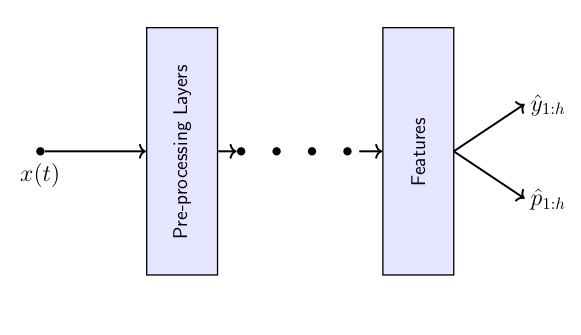
\includegraphics[width=0.5\textwidth]{figures/network.jpg}}
%\vspace{.3in}
%\caption{Network architecture}
%\label{fig:network}
%\end{figure}


In section \ref{sec:exp}, we use fully connected neural architectures having a maximum depth of 
two hidden layers, for prediction of outputs and time lags.

\section{Experiments}\label{sec:exp}


Just as the MNIST, CIFAR Santa Fe Laser and other data sets serve as a way to evaluate machine learning 
algorithms, it is necessary to propose benchmark problems for \emph{Probabilistic Dynamic Time Lag}.

This is particularly challenging given the nature of the PDT problem, although time lag 
relationships do exist in real world data sets (\cite{doi:10.1002/jgra.50429}, \cite{ZHOU2006195}), 
it is difficult to find data sets with time lag relationships explicitly annotated.

This barrier can be surpassed in turn by careful construction of synthetic data sets which incorporate 
dynamic time lag relationships between causes and effects with various complexity.

Synthetic data sets allow us to evaluate the accuracy of both, the output and time lag predictions of 
PDT models. To this end, we propose four benchmark tests, which are motivated by their connection 
to the solar wind prediction problem, but which we hope can become canonical examples in the area 
of PDT modelling.

\subsection{Data Generation}

We start by generating the time series $x(t) \in \mathbb{R}^8$, of size $4000$ 
(one copy for training and another for test), which represent the driving forces in our system. 
This can be achieved with good flexibility using \emph{Stochastic Langevin Dynamics} as shown in 
equation \ref{eq:data}.

\begin{align}
 x(t + 1) &= (1 - \tau) x(t) + \mathcal{N}(0, \sigma^2) \label{eq:data}\\
 y(t + \tau(t)) &= \alpha ||x(t)||^2 \label{eq:outputs}
\end{align}

In equation \ref{eq:outputs} we define the output $y(.)$ as the square norm of the appropriately 
time lagged input, where $\tau(t)$ determines the time lag relationship.

\subsection{Generating Predictions}

As described in section \ref{sec:model} above, for each input pattern $x(t)$, the model 
generates two sets of predictions, i.e. ${\hat{y}_i}$, output estimates and probabilities $\hat{p}_i$ 
for the time window $i \in [t+\ell, t+\ell+h)$ of width $h$. In all of the following benchmarks we set 
$\ell = 0$ and $h = 20$.

To evaluate the model predictions for the benchmarks, we choose the 
prediction $\hat{y}_j$ which has the highest probability of a causal link 
$j = {argmax}_{i} \ \hat{p}_i \ \ i \in [t+\ell, t+\ell+h)$. The predictions 
$(\hat{y}_j, j)$ can now be compared to their corresponding ground truth values 
$(y(t + \tau(t)), \tau(t))$. 

When generating predictions for temporally successive test patters $x'(t)$, it is possible that our 
model produces time gaps in the reconstruction of the test outputs $y'(t)$. This can happen due to 
departure from the assumptions outlined in section \ref{sec:formulation}. We can get around these 
gaps using linear interpolation.


\subsection{Benchmark Problems}\label{sec:benchmark}

Based on the above framework we construct four benchmark problems.

\begin{enumerate}
\item \textbf{Problem I} Constant Lag: \newline 
$\tau(t) = k$

\item \textbf{Problem II} Constant Velocity $\alpha ||x(t)||^2 + c$; Fixed Distance $d$: 
\newline $\tau(t) = d/(\alpha ||x(t)||^2 + c),\ \alpha = \frac{100}{8},\ d = 1000,\ c = 40$

\item \textbf{Problem III} Constant Acceleration $a$; Fixed Distance $d$: 
\newline $\tau(t) = (\sqrt{\alpha^2||x(t)||^4 + 2ad} - \alpha||x(t)||^2)/a,\ \alpha = \frac{50}{8},\ a = 5,\ d = 1000$

\item \textbf{Problem IV} Softplus time lag: 
\newline $\tau(t) = exp\left(||x(t)||^2\right)/\left(1 + exp(||x(t)||^2)\right)$

\end{enumerate}



\subsection{Results}

The results of the experiments of \ref{sec:benchmark} are evaluated using the following charts.

\begin{enumerate}
    \item Output-Time Lag charts: Since the output time lag relationship can be expressed in closed 
          form, we can visualize this relationship in the generated data sets and evaluate how well 
          the model is able to infer it.
    \item Error heat-maps: Heat maps of prediction error in velocity vs prediction error 
          in time lag. They help in visualizing the shape of the error distribution.
\end{enumerate}


\subsubsection{Problem I}

This is the simplest of the benchmark problems, the task is simply to learn a constant time lag from 
the training data. On the test data set for this problem, the model predicts the correct time lag for 
$99.92\%$ of the samples. 

With respect to prediction of the outputs, the model has a \emph{mean absolute error} (MAE) of 
$6.904677$ and achieves a Pearson correlation coefficient of $0.9795$ on a test data set in which the 
output lies in the range $[9.454, 290.550]$. It should be noted that the $y(t - 1)$ predictor 
achieves a MAE of $5.186521$ and a Pearson correlation of $0.991$ on this data set. The model is 
thus able to learn the input-output and time lag mappings easily for this problem.


\begin{figure*}
  \centering

  \begin{subfigure}[b]{0.4\textwidth}
    \centering
    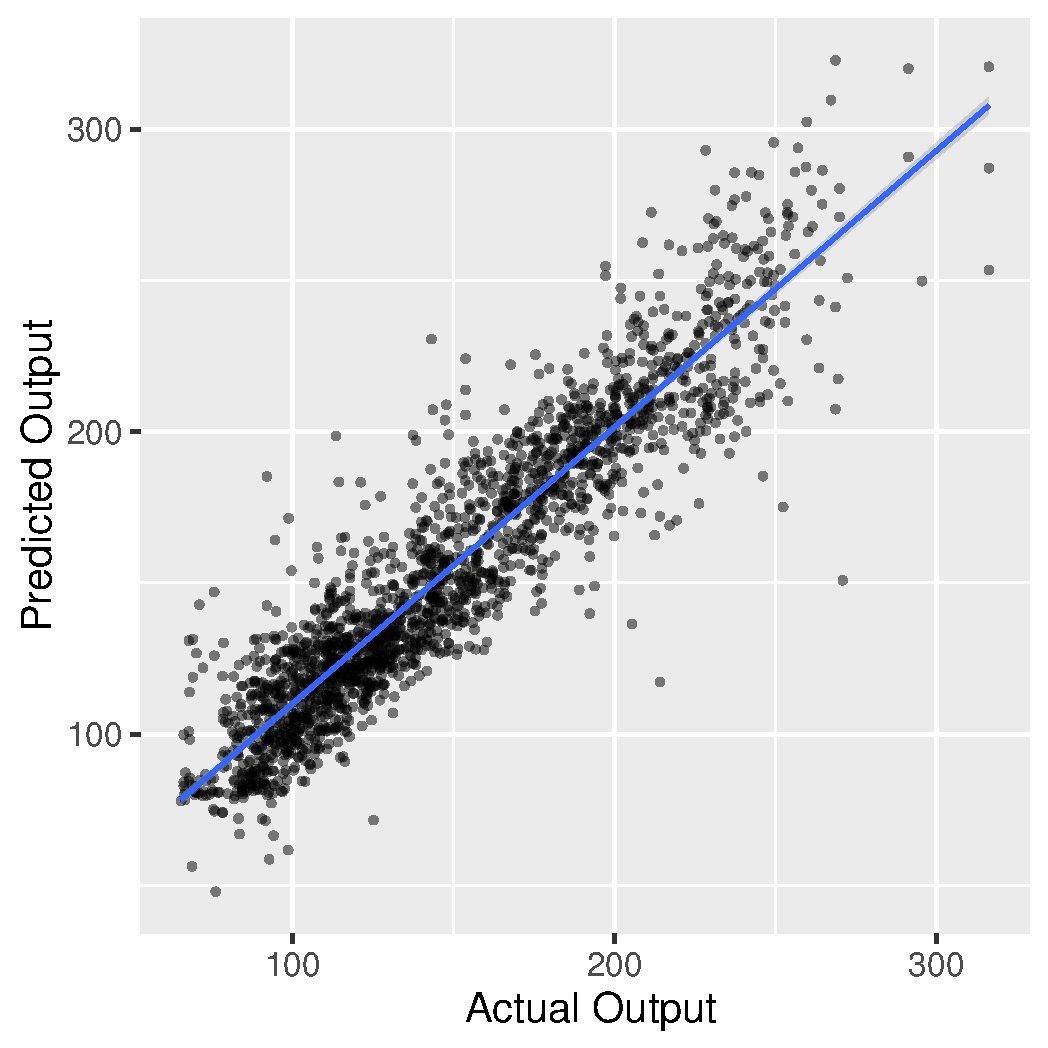
\includegraphics[width=\textwidth]{figures/exp2_scatter_v_test}
    \caption{ \textbf{Problem II}, Goodness of fit, Output $y(x)$}
    \label{fig:problem2_fitv}
  \end{subfigure}
  \hfill
  \begin{subfigure}[b]{0.4\textwidth}
    \centering
    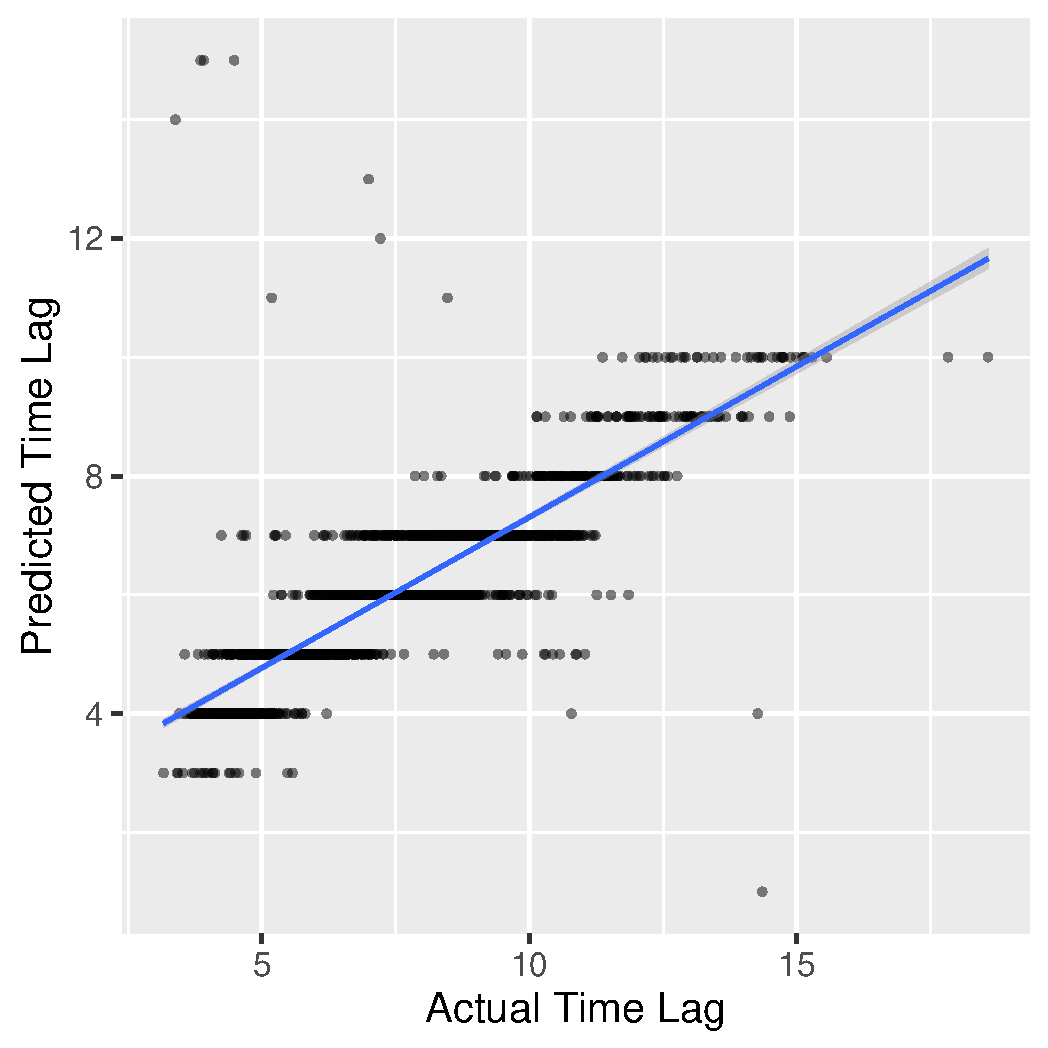
\includegraphics[width=\textwidth]{figures/exp2_scatter_t_test}
    \caption{ \textbf{Problem II}, Goodness of fit, Timalag $\tau(t)$ }
    \label{fig:problem2_fitt}
  \end{subfigure}
  
  \vskip\baselineskip
  
  \begin{subfigure}[b]{0.4\textwidth}
    \centering
    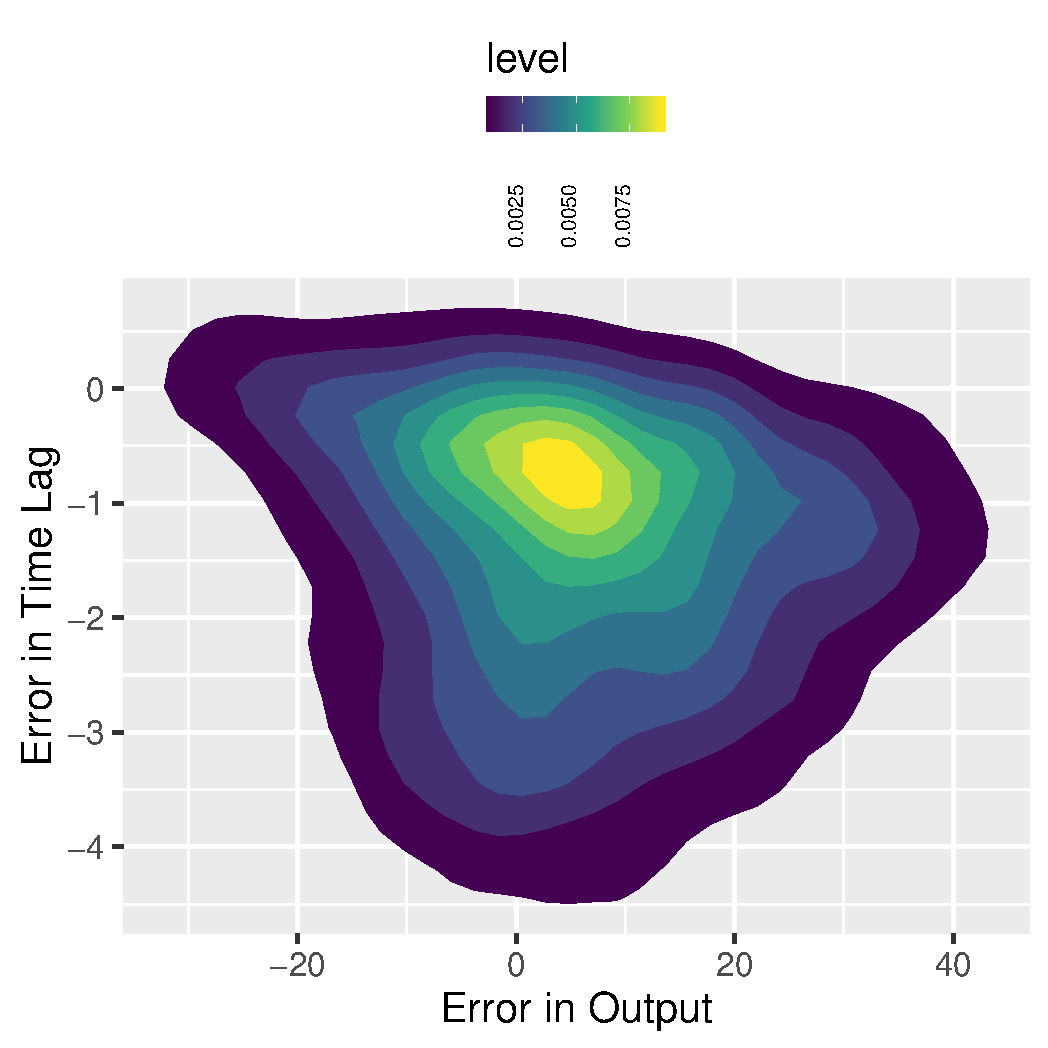
\includegraphics[width=\textwidth]{figures/exp2_errors}
    \caption{ \textbf{Problem II}, Error in prediction of output vs error in time lag prediction} 
    \label{fig:problem2_error}
  \end{subfigure}
  \hfill
  \begin{subfigure}[b]{0.4\textwidth}
    \centering
    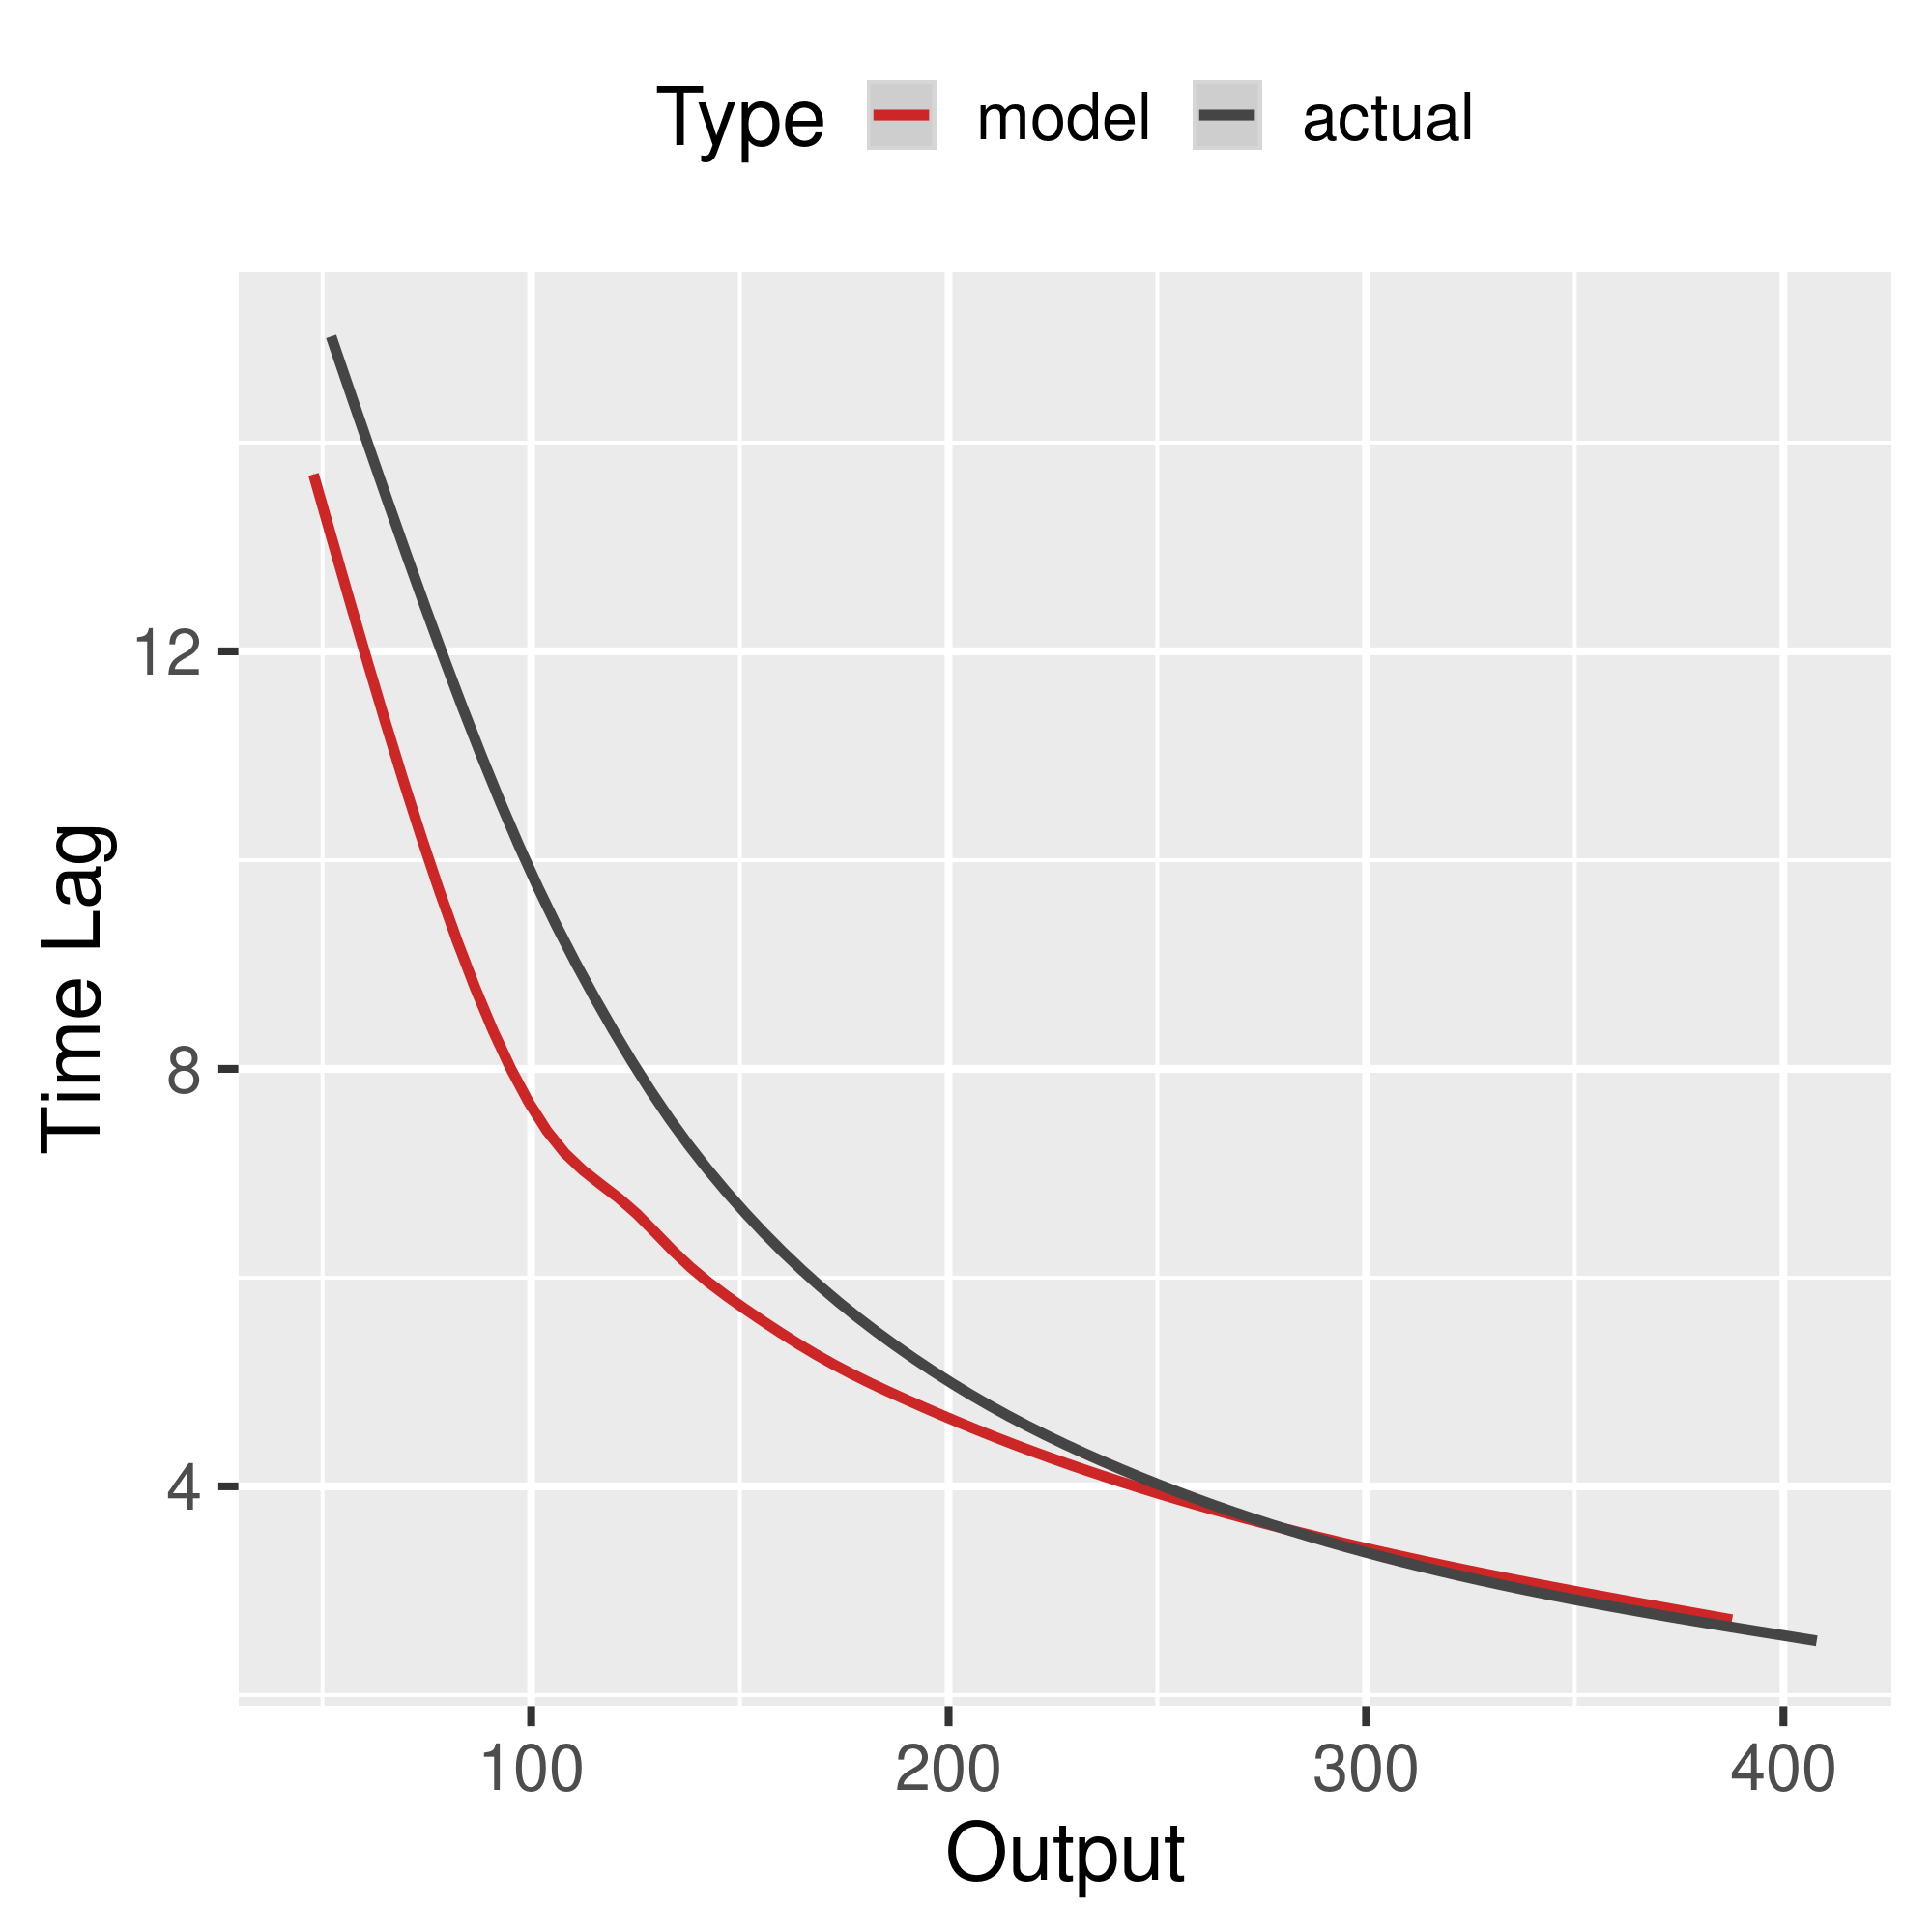
\includegraphics[width=\textwidth]{figures/exp2_predictive_curves}
    \caption{ \textbf{Problem II}, Output vs Time Lag Relationship} 
    \label{fig:problem2_curves}
  \end{subfigure}

  \vskip\baselineskip
  
  \begin{subfigure}[b]{0.4\textwidth}
    \centering
    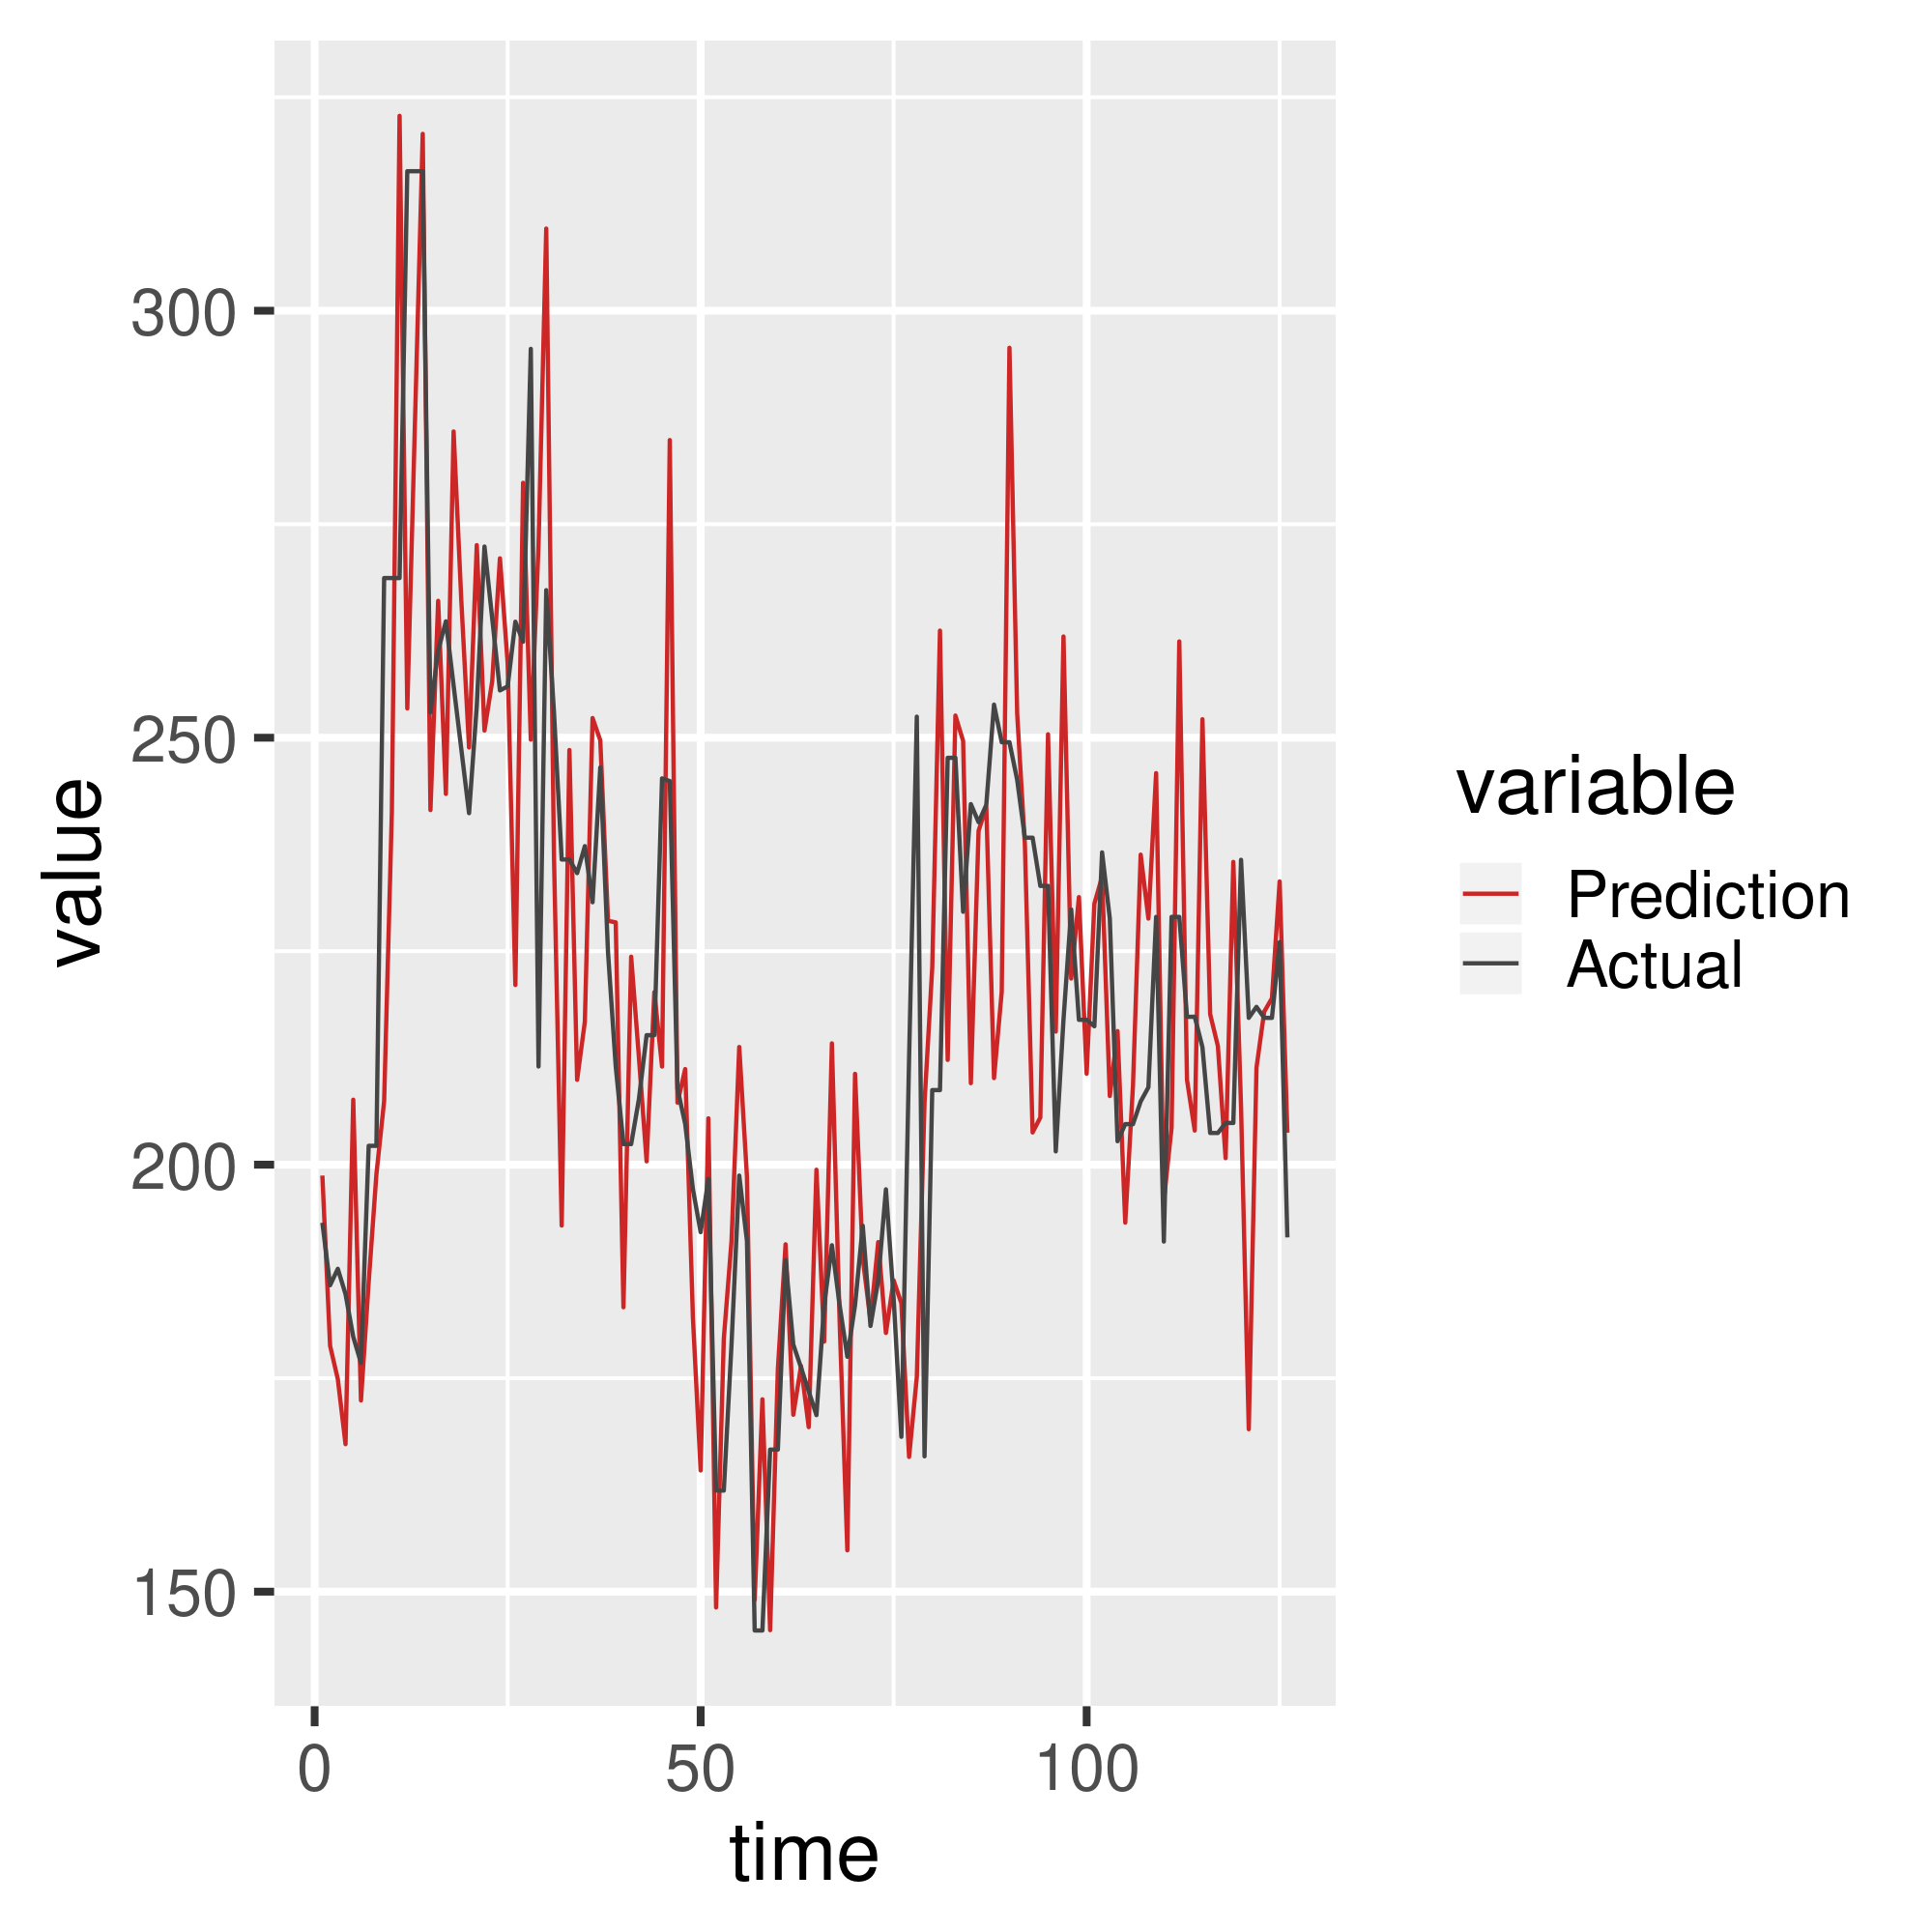
\includegraphics[width=\textwidth]{figures/exp2_timeseries_pred}
    \caption{ \textbf{Problem II}, A portion of the test time series reconstructed using the model} 
    \label{fig:problem2_timeseries}
  \end{subfigure}
  \hfill
  \begin{subfigure}[b]{0.4\textwidth}
    \centering
    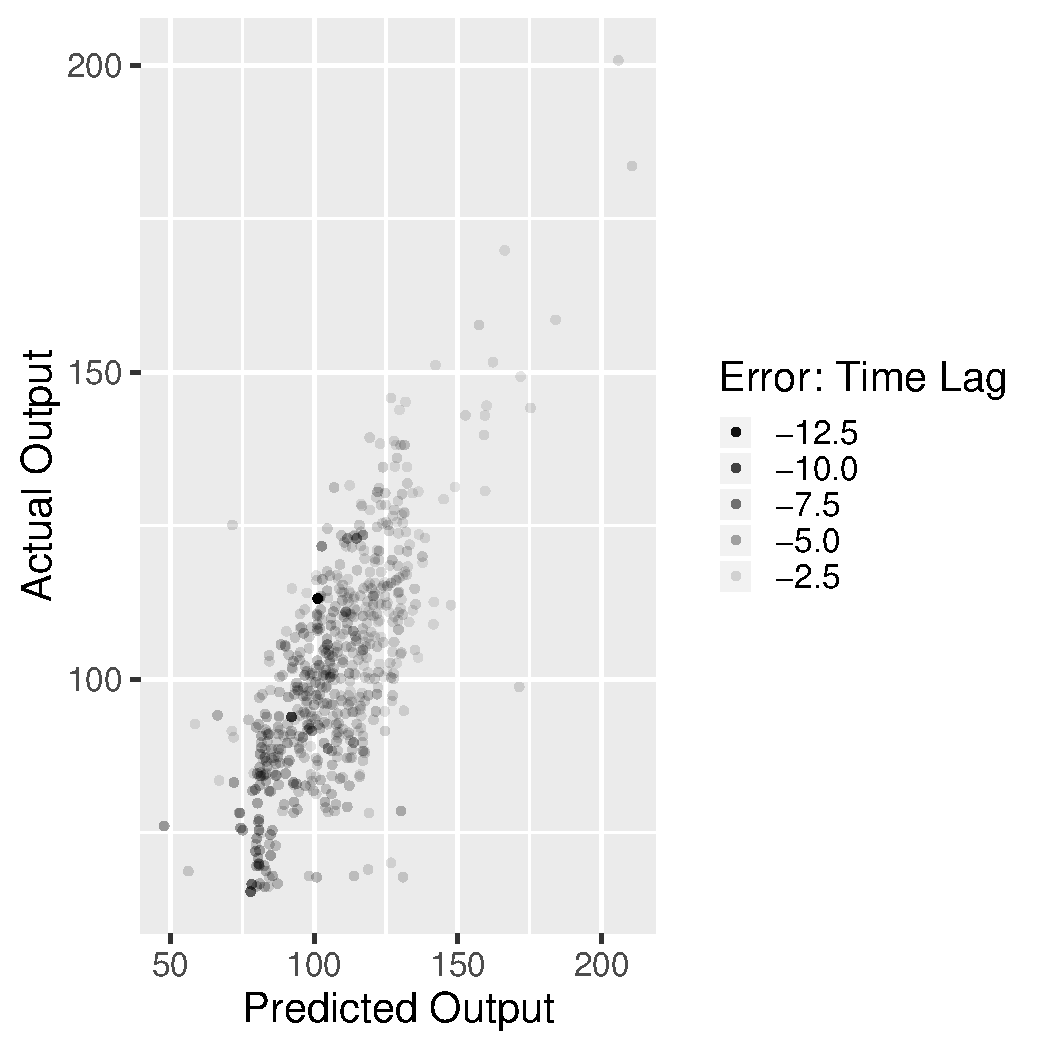
\includegraphics[width=\textwidth]{figures/exp2_lag_error_jus}
    \caption{ \textbf{Problem II}, Predicted vs Actual Outputs for the cases with time lag error $\leq -2.5$.} 
    \label{fig:problem2_lag_error_jus}
  \end{subfigure}
  
  \caption{\textbf{Problem II}, Results}
\end{figure*}




\subsubsection{Problem II}

Figures \ref{fig:problem2_fitv} and \ref{fig:problem2_fitt} shows scatter plots between the output value and associated 
time lag, it compares the scatter distribution generated by the model and compares it with the 
distribution seen in the test data.

In figure \ref{fig:problem2_error} we present a scatter plot which shows the distribution of the 
errors in output versus the error in time lag predictions.

In figure \ref{fig:problem2_curves} we present smoothed trends extracted from the data presented in 
\ref{fig:problem2_fitv}, the red curve represents the output time lag function learned by the model 
while the black curve is the \emph{ground truth} dependence between the two. 

We can see that the model is able to approximate the inverse relationship between the output and 
time lag from the training data.


\begin{figure*}
  \centering

  \begin{subfigure}[b]{0.4\textwidth}
    \centering
    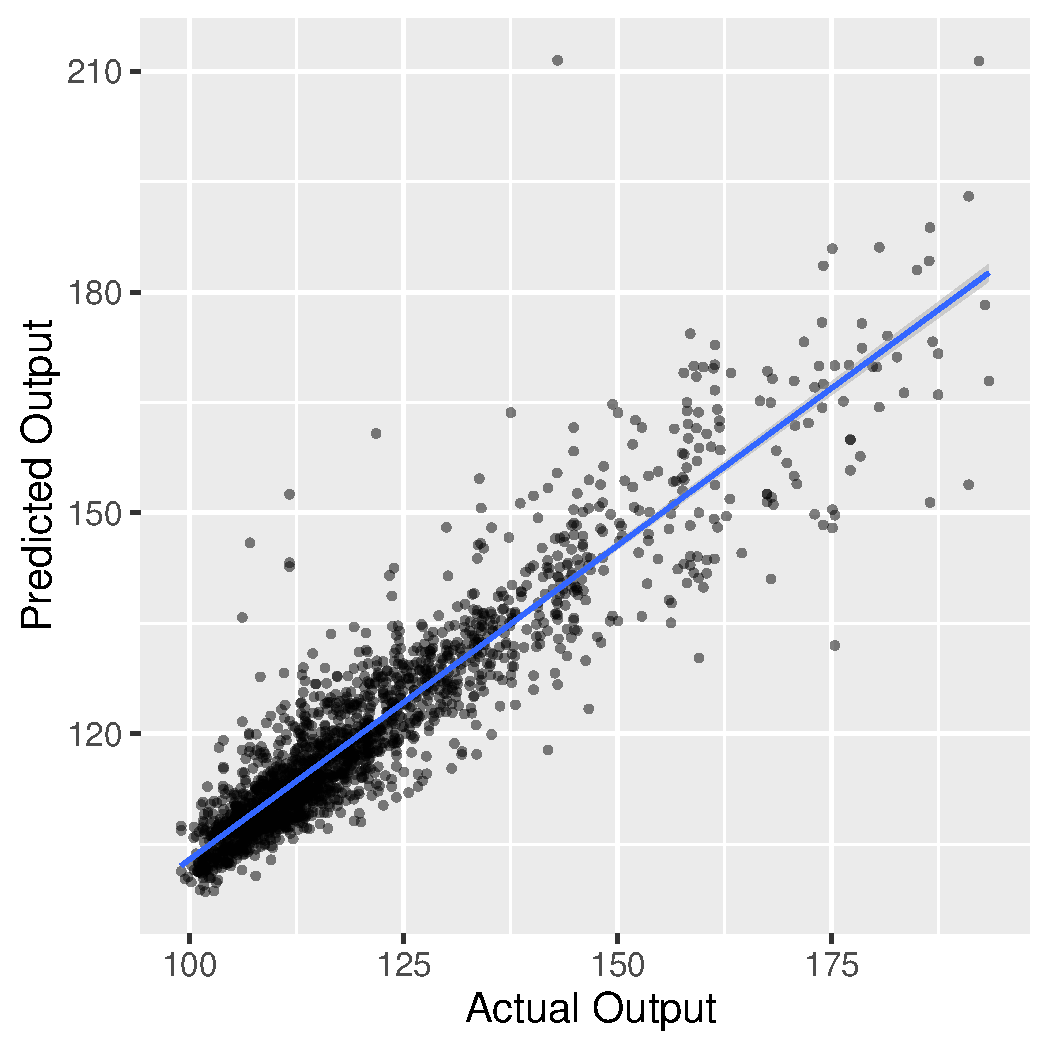
\includegraphics[width=\textwidth]{figures/exp3_scatter_v_test}
    \caption{ \textbf{Problem III}, Goodness of fit, Output $y(x)$}
    \label{fig:problem3_fitv}
  \end{subfigure}
  \hfill
  \begin{subfigure}[b]{0.4\textwidth}
    \centering
    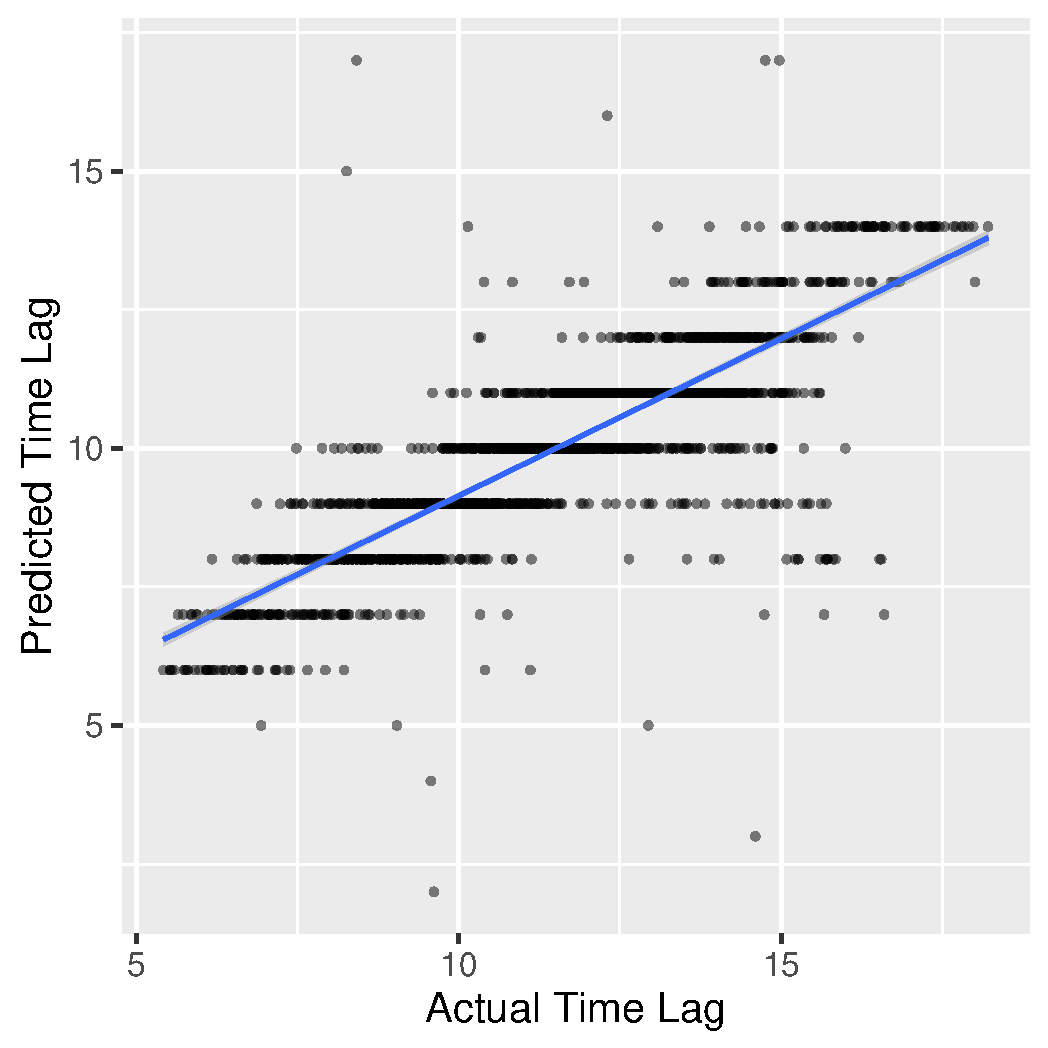
\includegraphics[width=\textwidth]{figures/exp3_scatter_t_test}
    \caption{ \textbf{Problem III}, Goodness of fit, Time lag $\tau(t)$ }
    \label{fig:problem3_fitt}
  \end{subfigure}

  \vskip\baselineskip
  
  \begin{subfigure}[b]{0.4\textwidth}
    \centering
    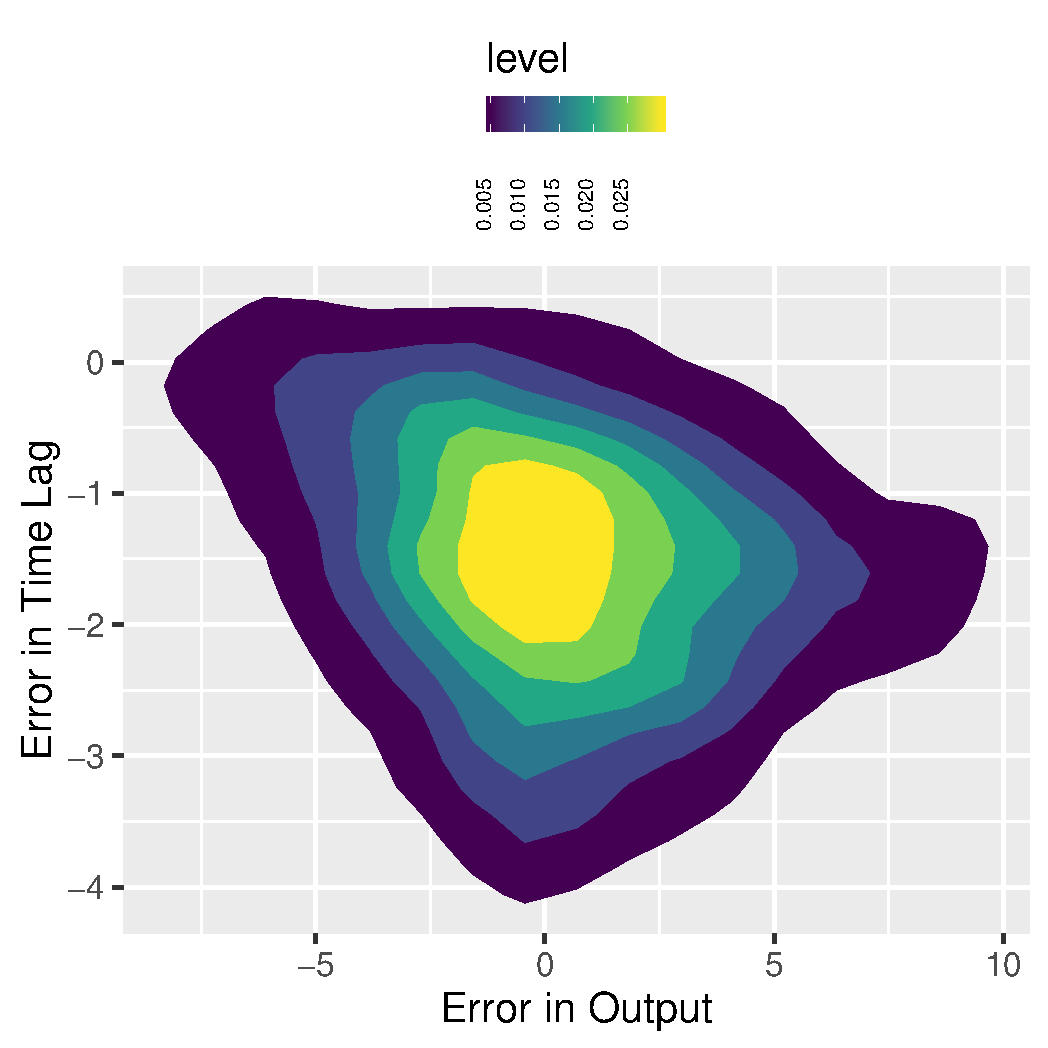
\includegraphics[width=\textwidth]{figures/exp3_errors}
    \caption{ \textbf{Problem III}, Error in prediction of output vs error in time lag prediction} 
    \label{fig:problem3_error}
  \end{subfigure}
  \hfill
  \begin{subfigure}[b]{0.4\textwidth}
    \centering
    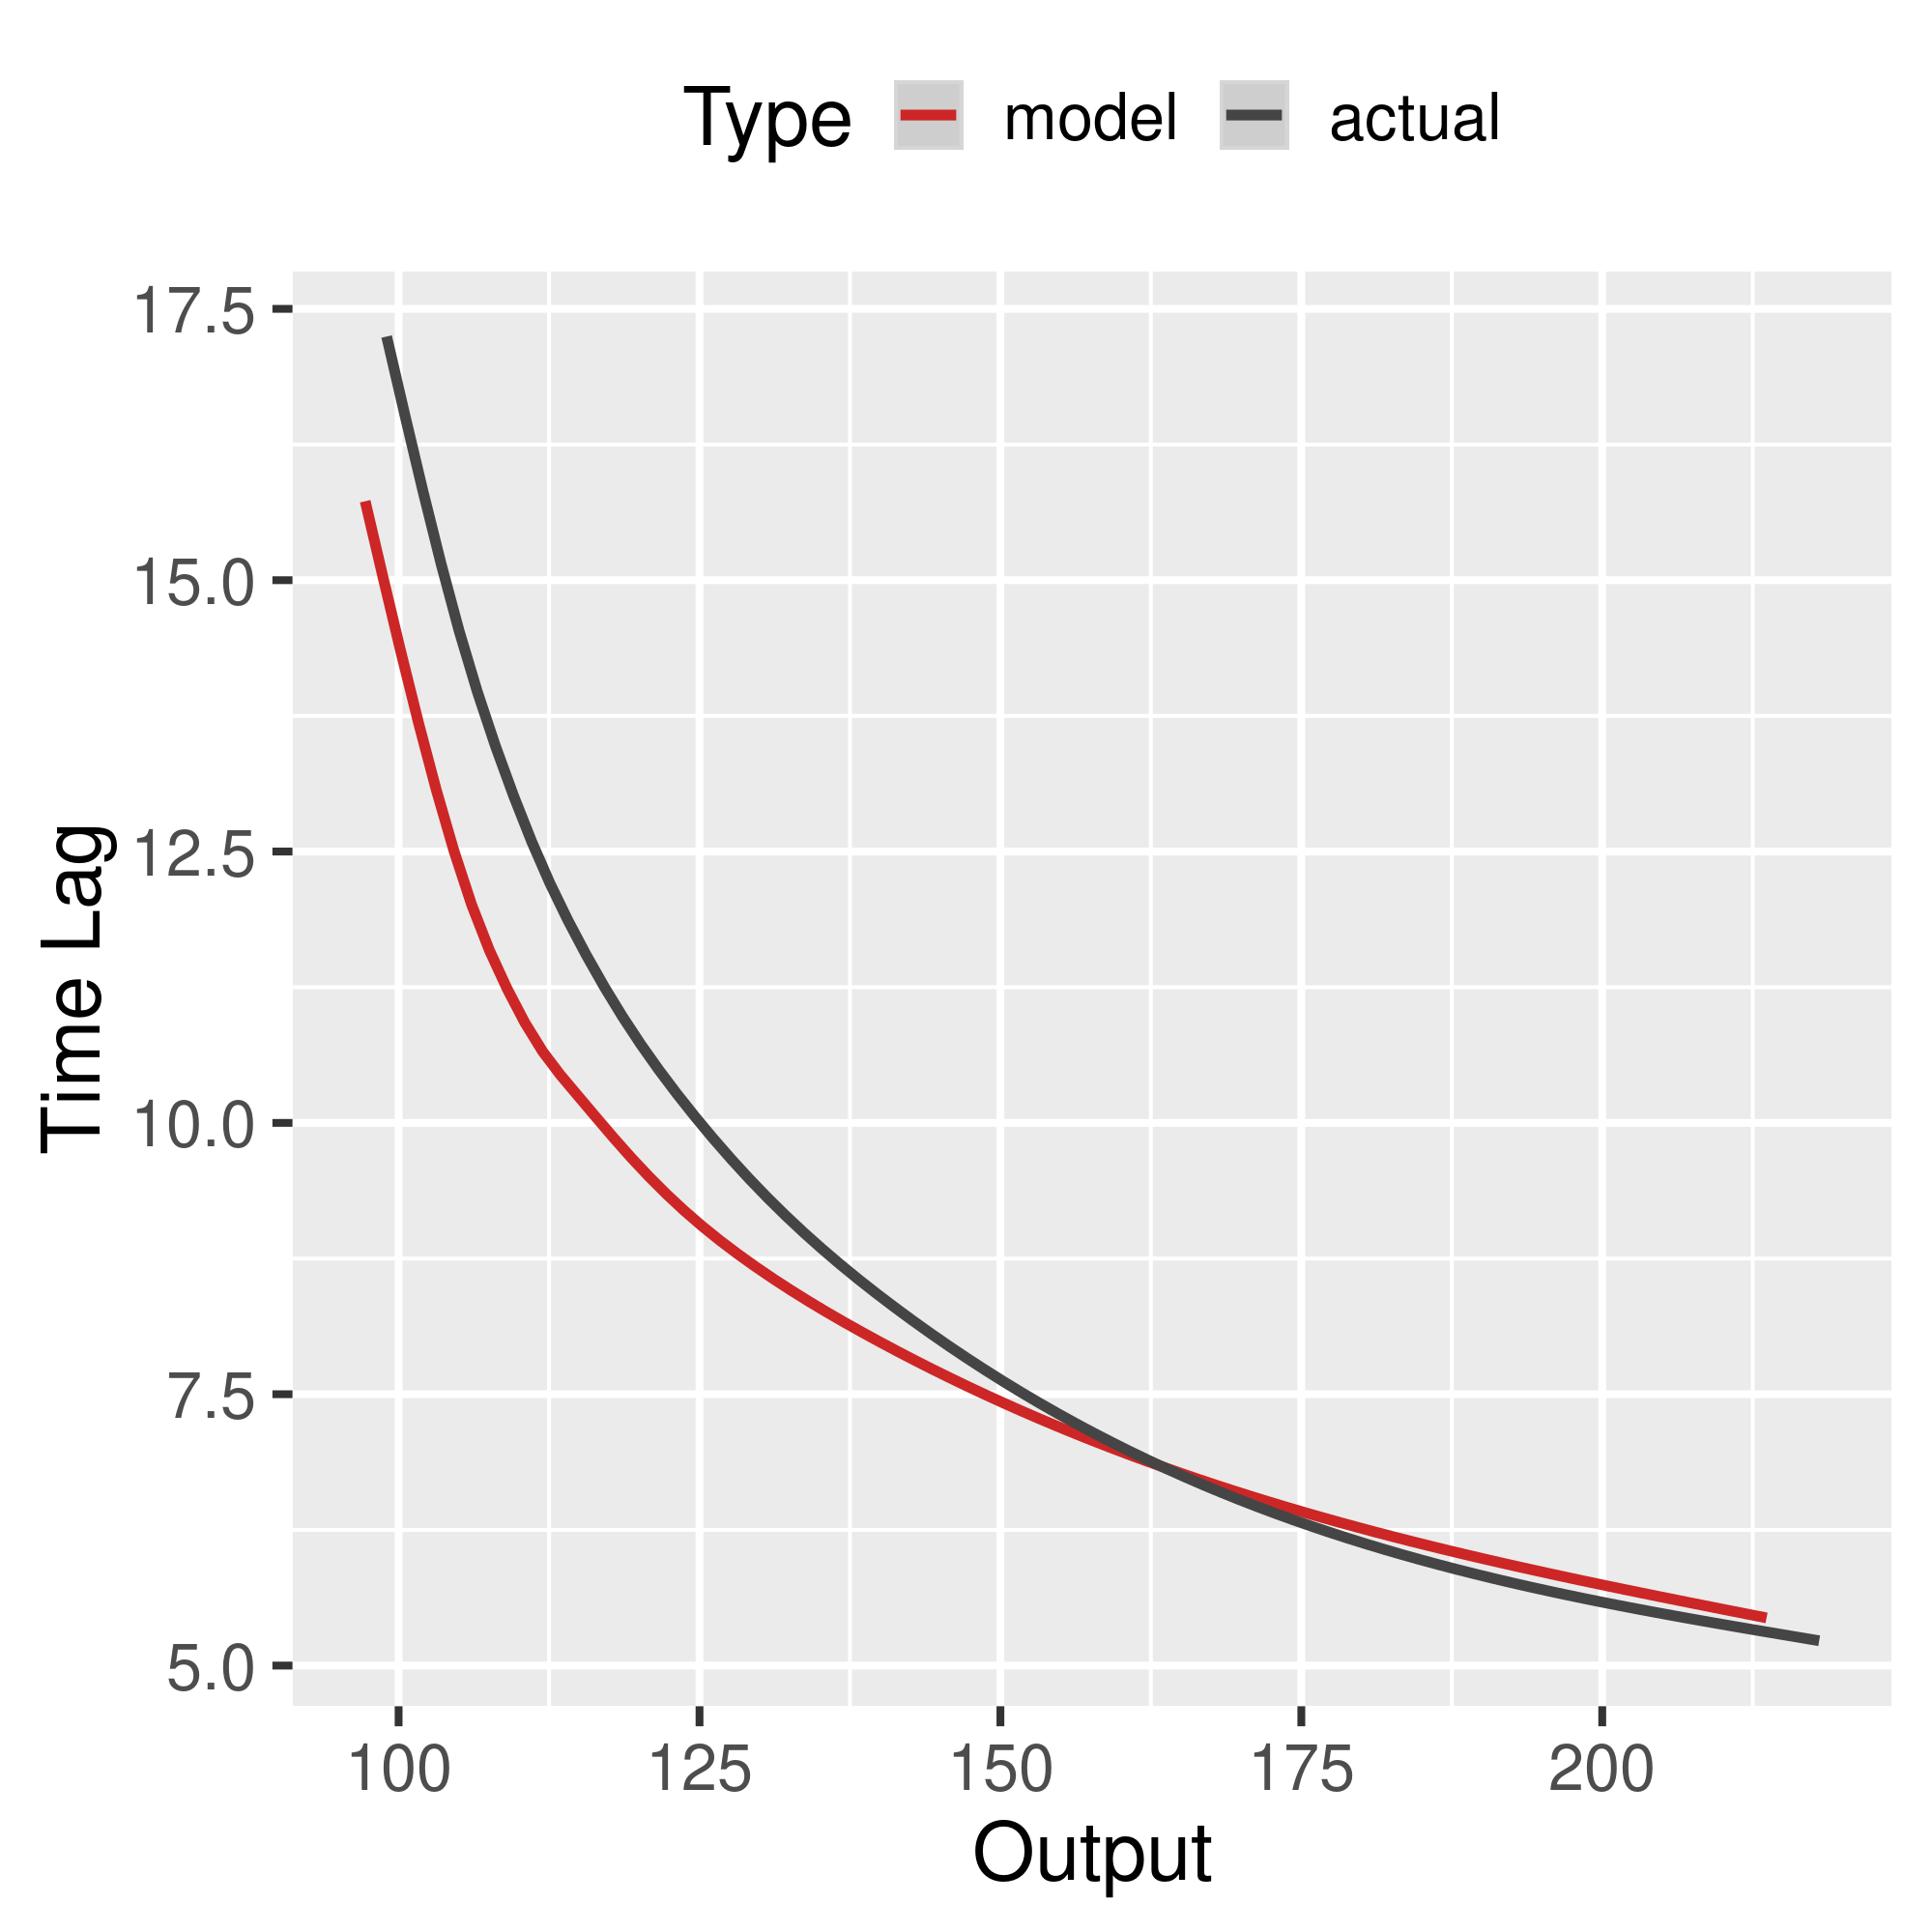
\includegraphics[width=\textwidth]{figures/exp3_predictive_curves}
    \caption{ \textbf{Problem III}, Output vs Time Lag Relationship} 
    \label{fig:problem3_curves}
  \end{subfigure}
  
  \vskip\baselineskip
  
  \begin{subfigure}[b]{0.4\textwidth}
    \centering
    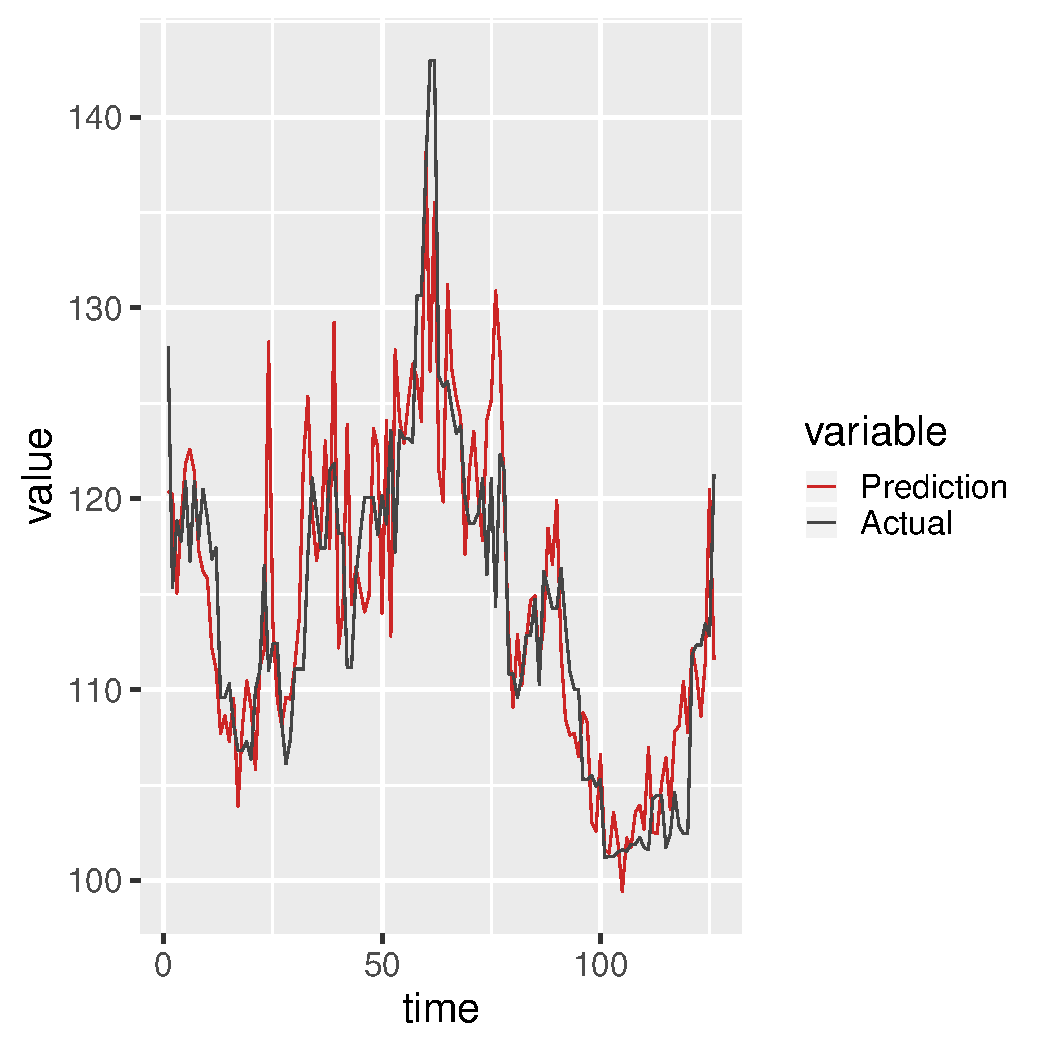
\includegraphics[width=\textwidth]{figures/exp3_timeseries_pred}
    \caption{ \textbf{Problem III}, A portion of the test time series reconstructed using the model} 
    \label{fig:problem3_timeseries}
  \end{subfigure}
  \hfill
  \begin{subfigure}[b]{0.4\textwidth}
    \centering
    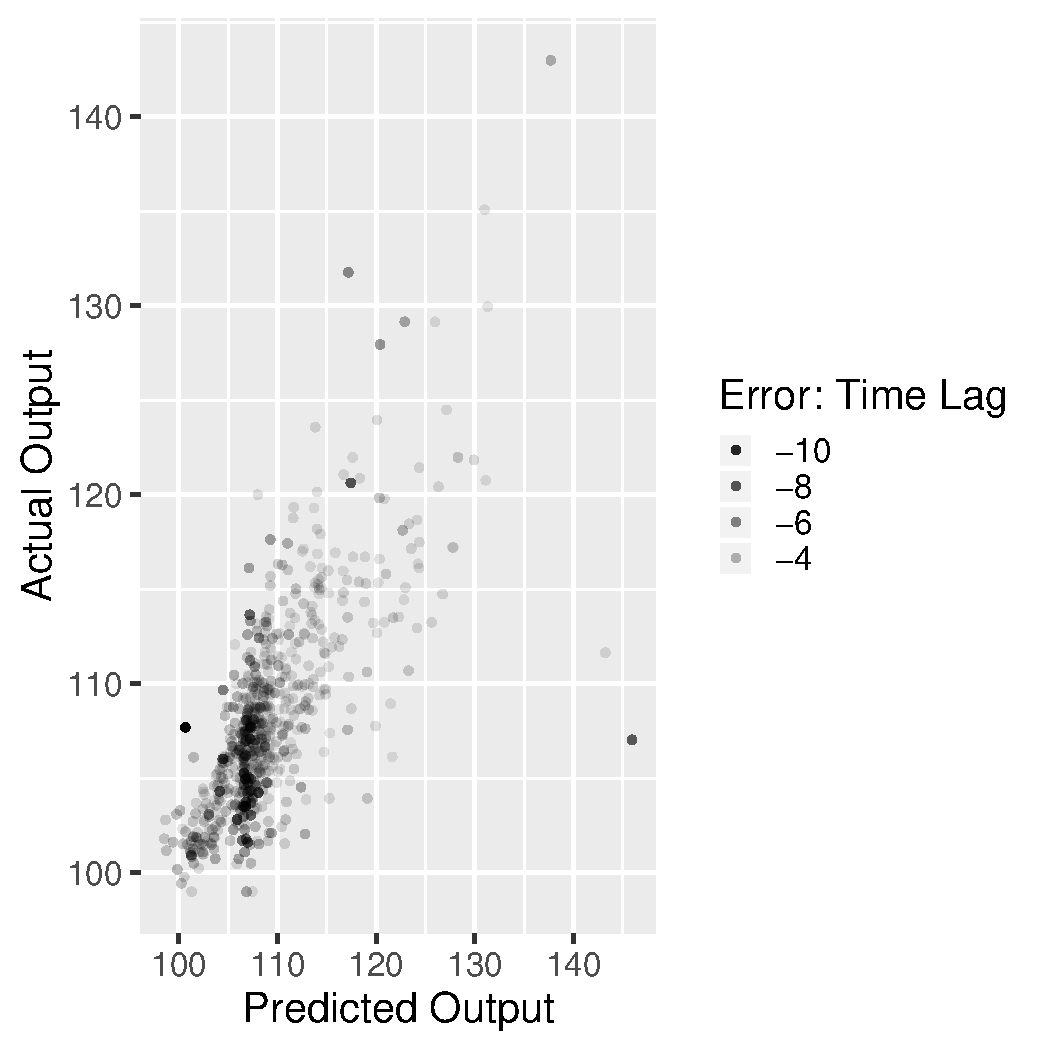
\includegraphics[width=\textwidth]{figures/exp3_lag_error_jus}
    \caption{ \textbf{Problem III}, Predicted vs Actual Outputs for the cases with time lag error $\leq -2.5$.} 
    \label{fig:problem3_lag_error_jus}
  \end{subfigure}
  
  \caption{\textbf{Problem III}, Results}
\end{figure*}


\subsubsection{Problem III}

Problem III involves a more complicated output time lag relationship than problem II due to the 
effect of acceleration. From figures \ref{fig:problem3_fitv} and \ref{fig:problem3_fitv}, 
it can be observed that the model can still learn the time lag and output mappings although 
in this case the time lag error distribution has a slightly longer tail in figure 
\ref{fig:problem3_error} as compared to \ref{fig:problem2_error}.

One observation common to the results of problems II and III is that the error distribution of 
the time lag is asymmetric, the model tends to underestimate the time lag. Upon closer examination 
of the predictions (figure \ref{fig:problem3_lag_error_jus}), it is observed that the data patterns 
for which the model has a time lag prediction error $\leq -2.5$, tend to occur in lower region of 
the output space. %(table \ref{table:problem3_stats}).

It is thus the case that for applications where there is an inverse relationship between the output 
and time lag, the model's time lag errors are expected to be biased towards the negative region, 
but when output and time lag are positively correlated, the time lag errors should be unbiased.


%\begin{table}[h]
%\caption{\textbf{Problem III}: Statistics of the Output distribution} \label{table:problem3_stats}
%\begin{center}
%\begin{tabular}{ll}
%\textbf{Statistic}  &\textbf{Value} \\
%\hline \\
%Minimum         & $111.7$ \\
%$1$st Quartile  & $182.3$ \\
%Median          & $252.1$ \\
%$3$rd Quartile  & $334.5$ \\
%Maximum         & $687.4$ \\
%\end{tabular}
%\end{center}
%\end{table}


\subsubsection{Problem IV}

Figures \ref{fig:problem4_fitv}, \ref{fig:problem4_fitt}, \ref{fig:problem4_curves} summarize 
the results of the experiment. This case is different as compared to the previous problems as there 
is now a monotonic relationship between the output and time lag. A key difference in the model 
performance in this problem can be observed in error scatter chart \ref{fig:problem4_curves}, 
we can see that the time lag errors are symmetric.


\begin{figure*}
  \centering

  \begin{subfigure}[b]{0.4\textwidth}
    \centering
    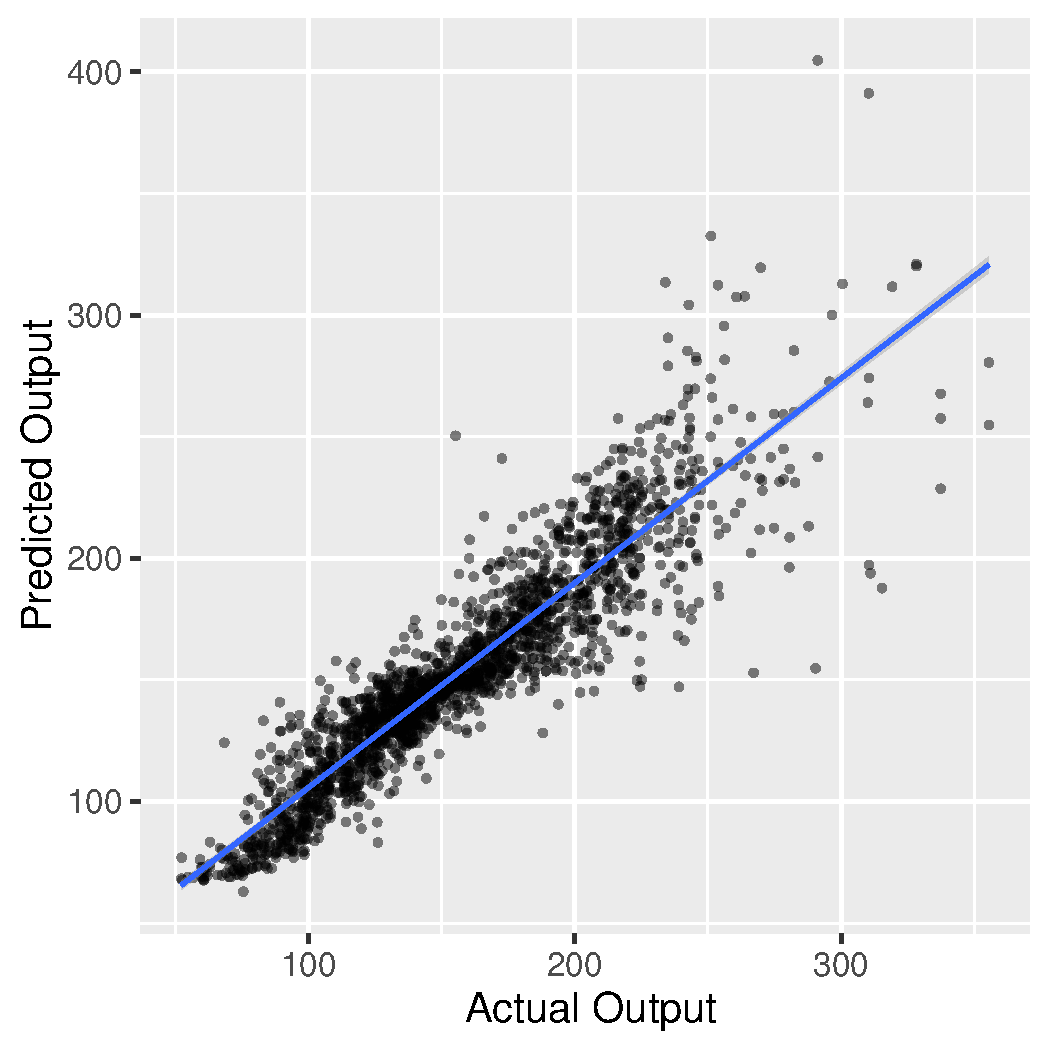
\includegraphics[width=\textwidth]{figures/exp4_scatter_v_test}
    \caption{ \textbf{Problem IV}, Goodness of fit, Output $y(x)$}
    \label{fig:problem4_fitv}
  \end{subfigure}
  \hfill
  \begin{subfigure}[b]{0.4\textwidth}
    \centering
    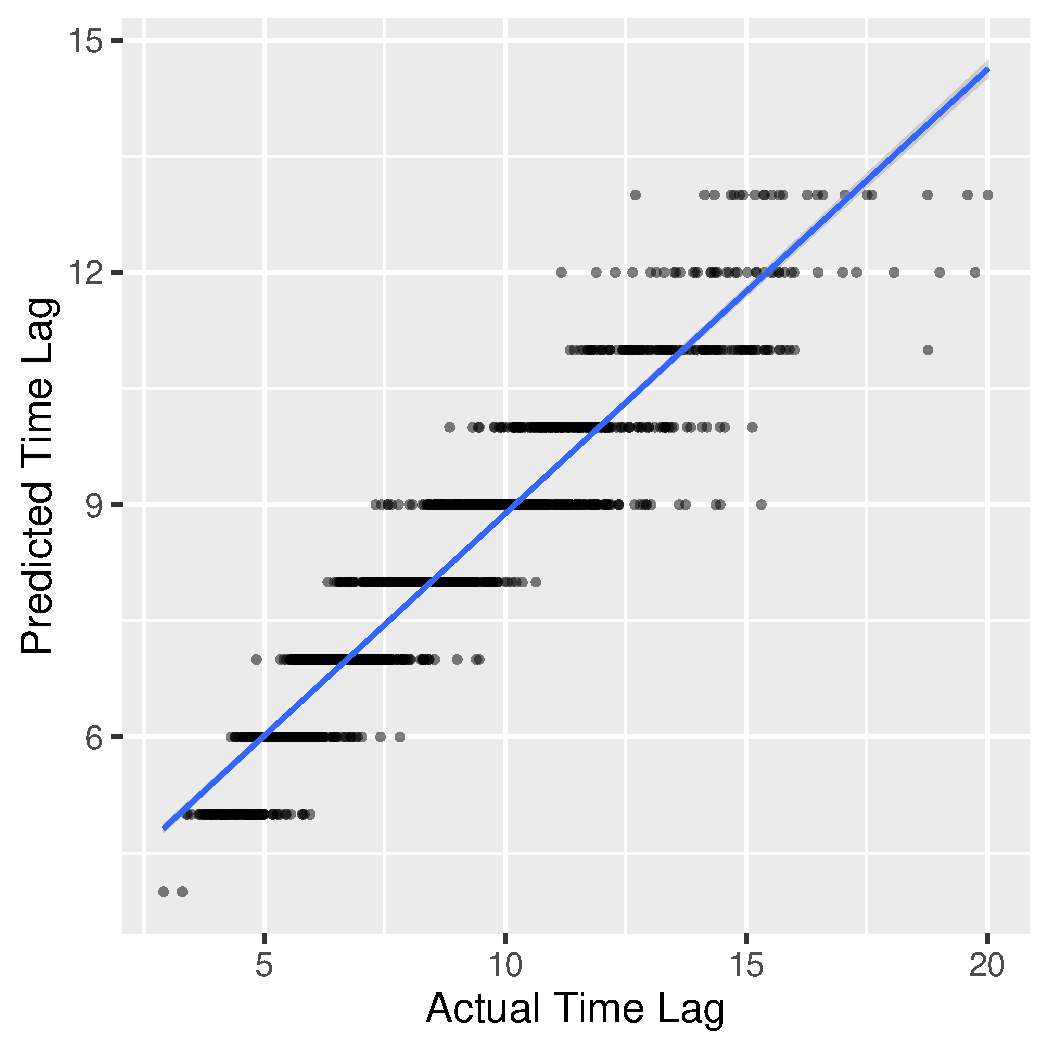
\includegraphics[width=\textwidth]{figures/exp4_scatter_t_test}
    \caption{ \textbf{Problem IV}, Goodness of fit, Time lag $\tau(t)$ }
    \label{fig:problem4_fitt}
  \end{subfigure}
  
  \vskip\baselineskip
  
  \begin{subfigure}[b]{0.4\textwidth}
    \centering
    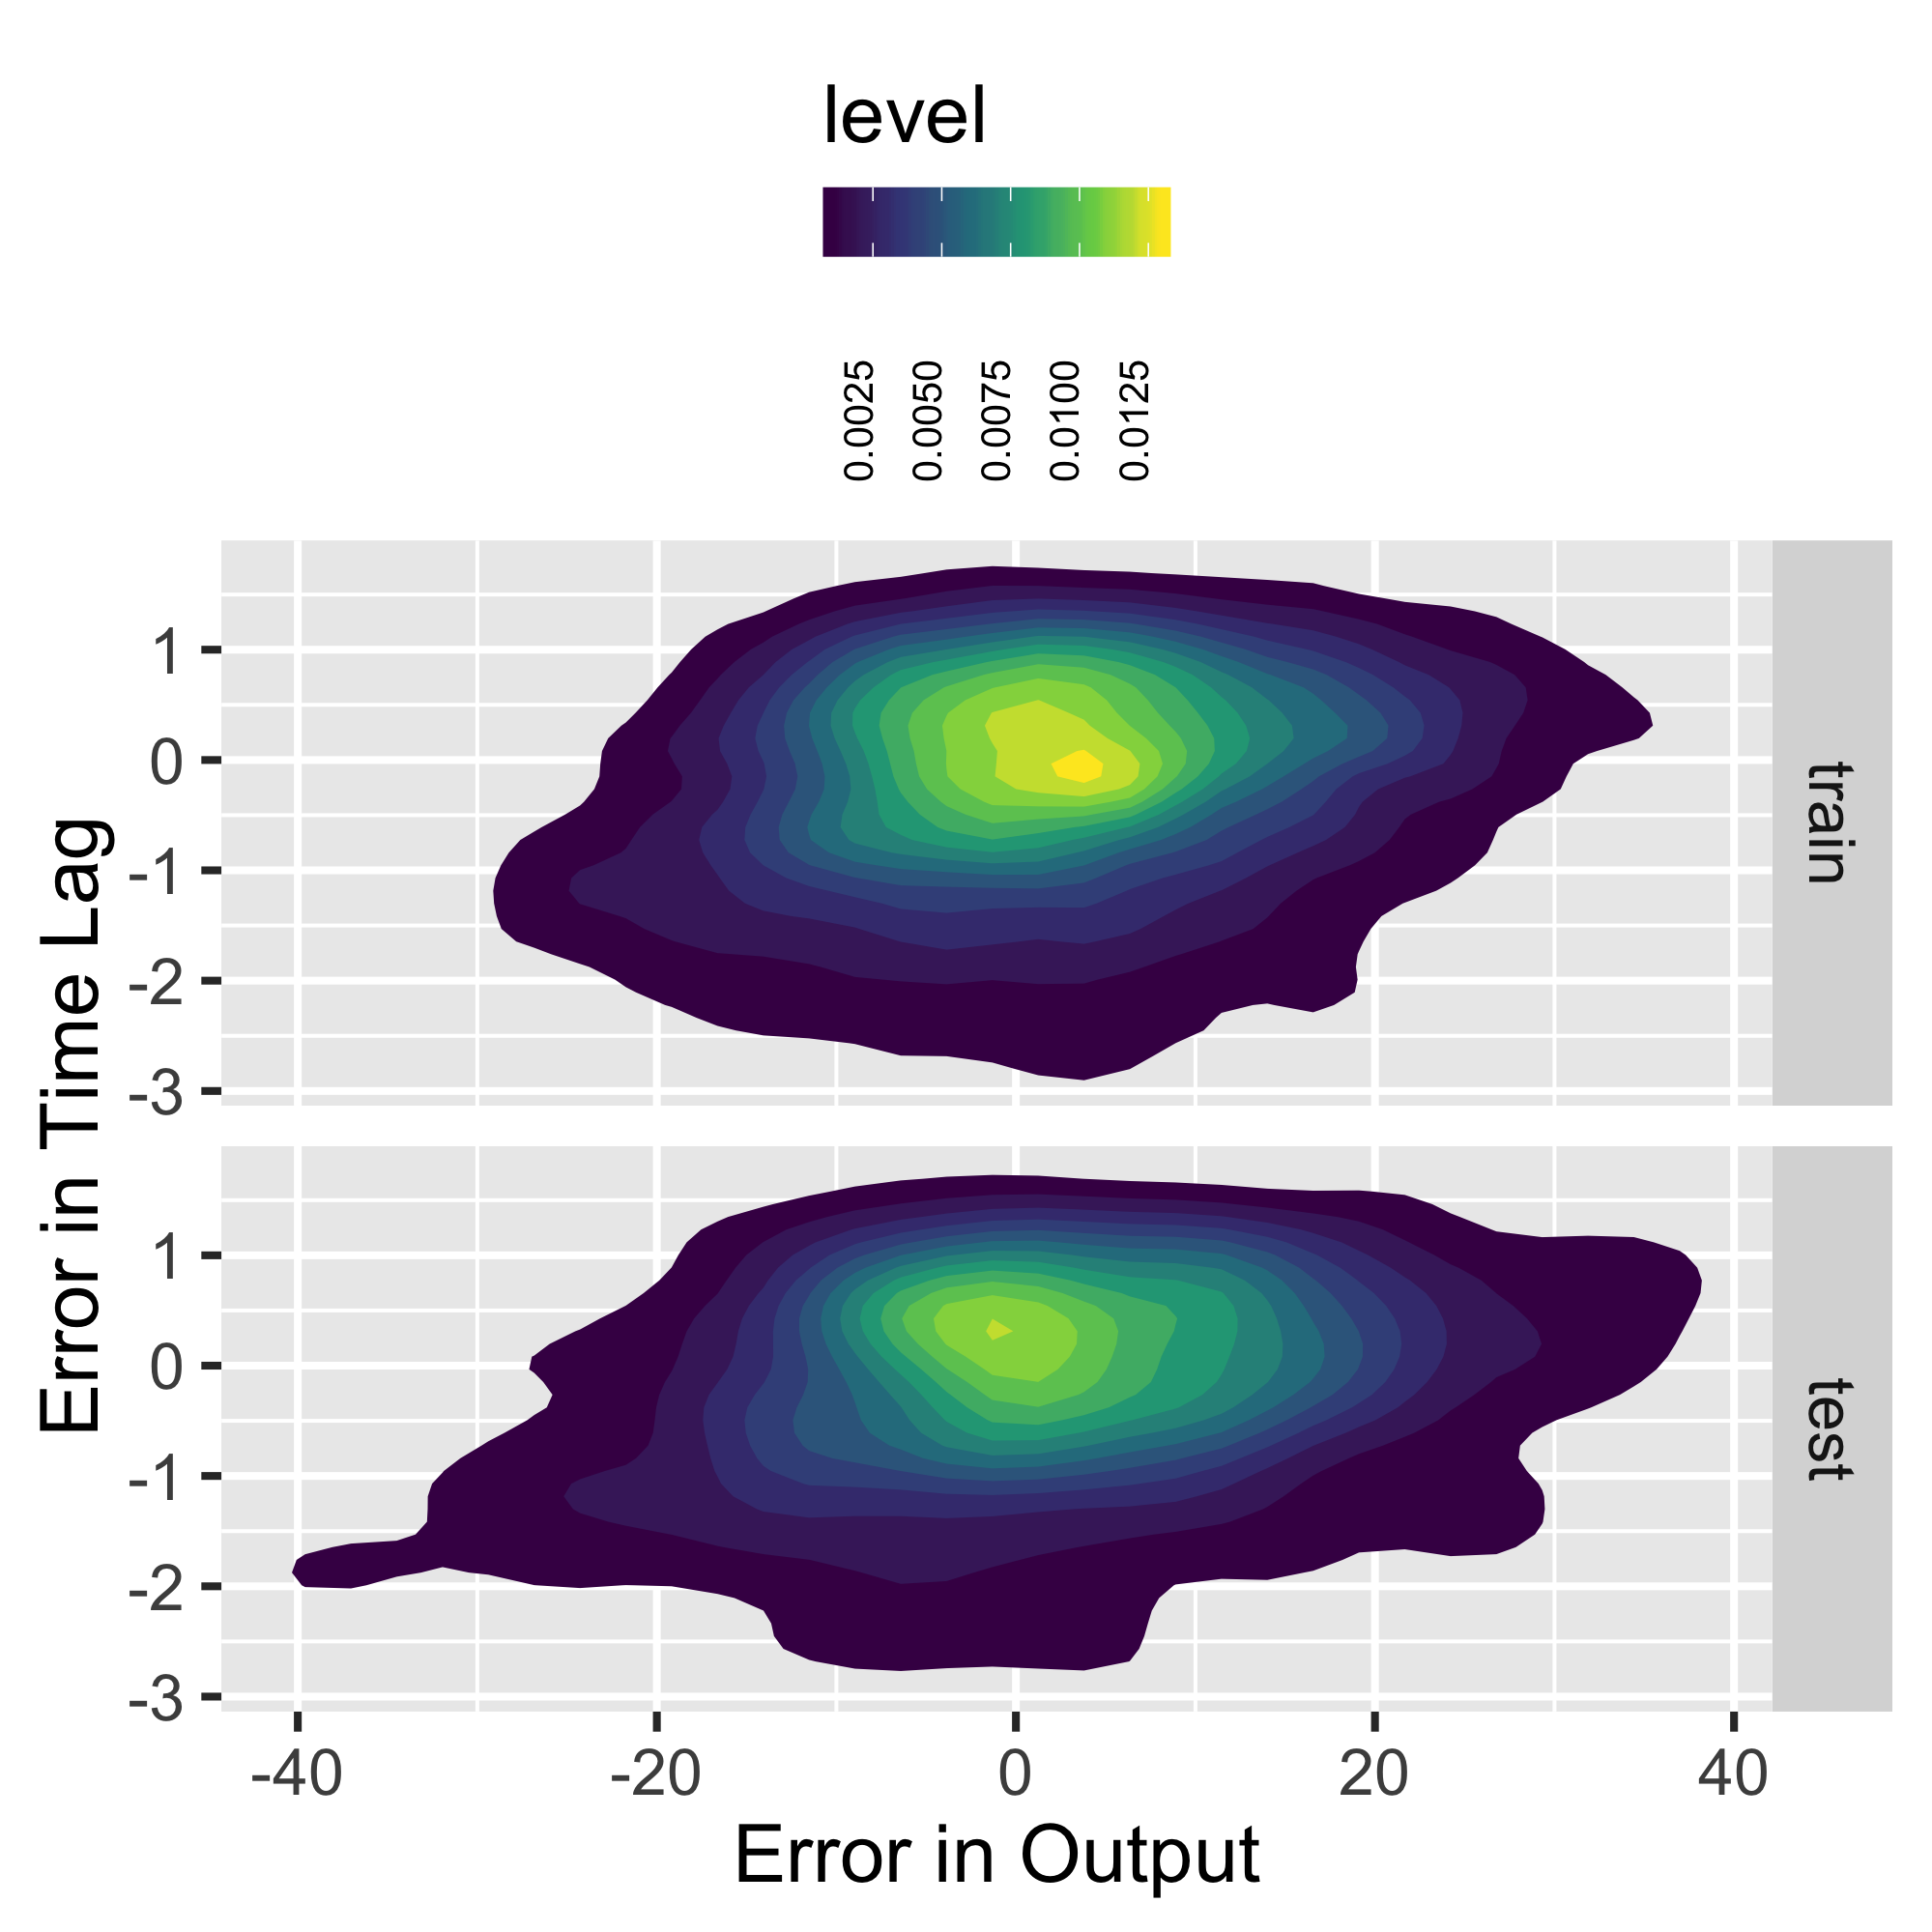
\includegraphics[width=\textwidth]{figures/exp4_errors}
    \caption{ \textbf{Problem IV}, Error in prediction of output vs error in time lag prediction} 
    \label{fig:problem4_error}
  \end{subfigure}
  \hfill
  \begin{subfigure}[b]{0.4\textwidth}
    \centering
    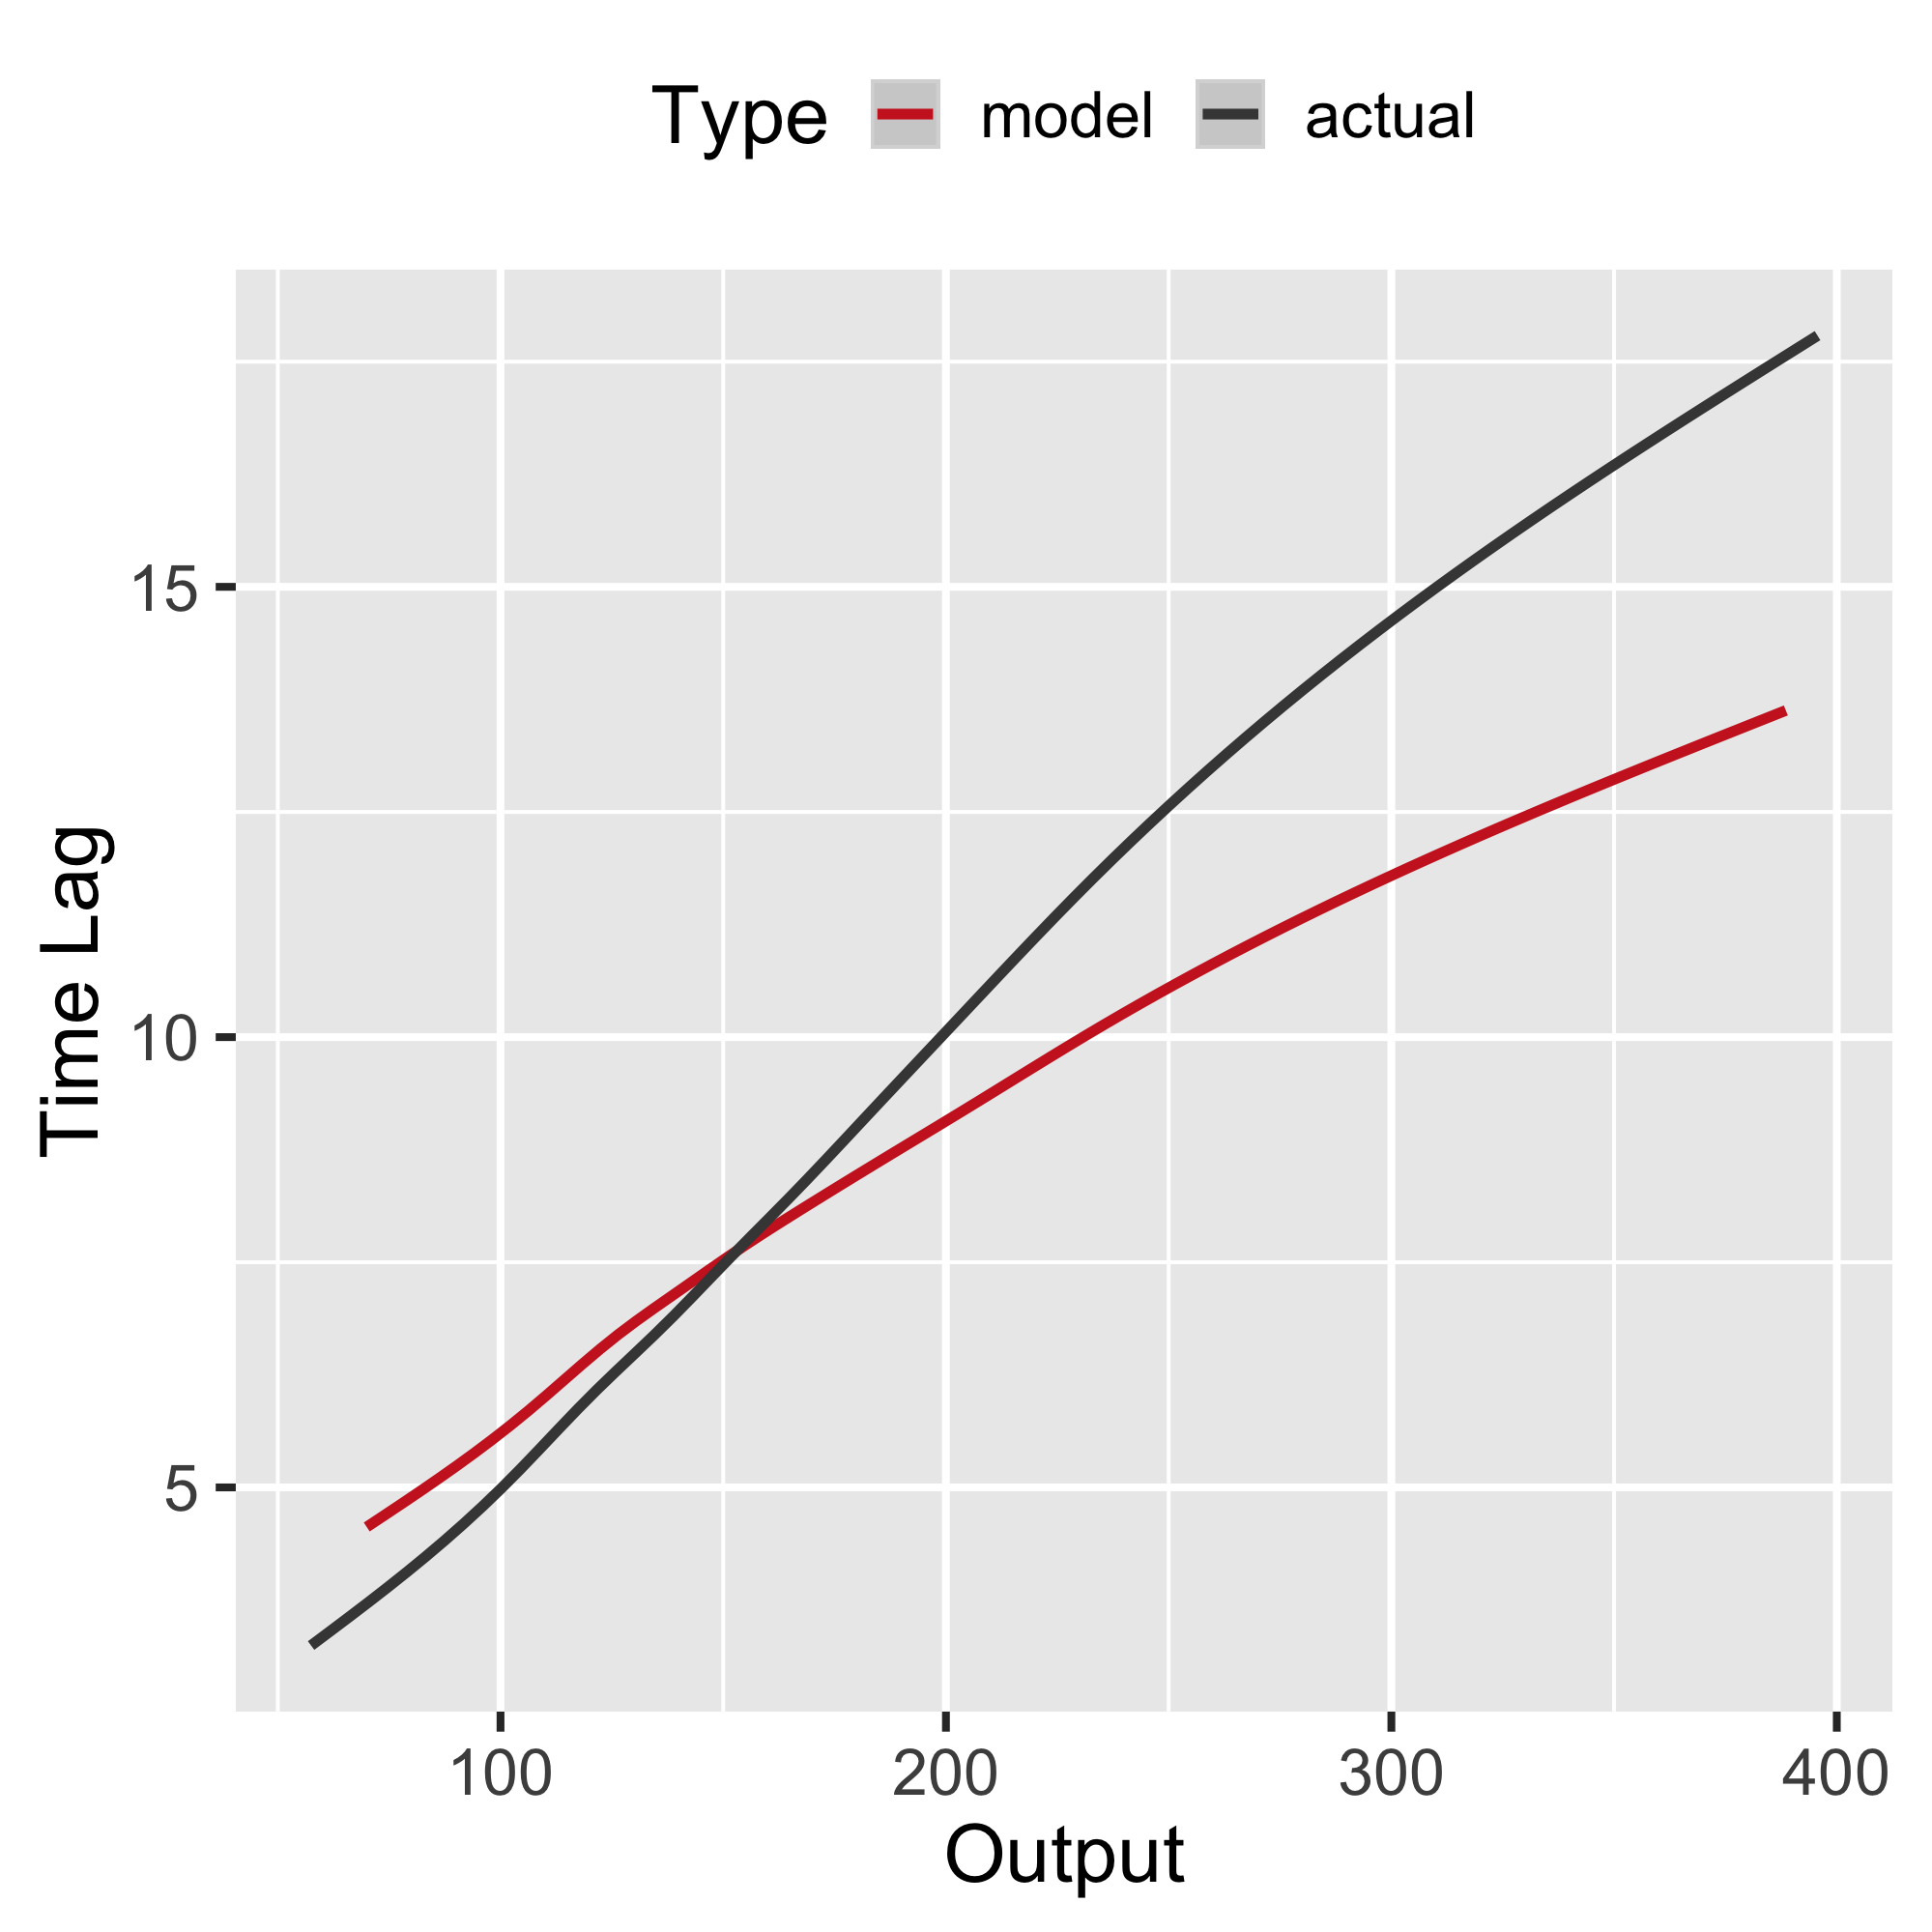
\includegraphics[width=\textwidth]{figures/exp4_predictive_curves}
    \caption{ \textbf{Problem IV}, Output vs Time Lag Relationship} 
    \label{fig:problem4_curves}
  \end{subfigure}
  
  \caption{\textbf{Problem IV}, Results}
\end{figure*}

\section{Conclusions}

We present in this work a formulation and a novel solution methodology for the problem of performing 
inference and forecasting in the context of lagged causal relationships between time series. 
We call this problem \emph{Probabilistic Dynamic Time Lag} (PDT) to note the non-stationary nature of the 
causal link between time series $x(t)$ and $y(t)$. We outline a neural network based solution to this 
problem and benchmark its performance on a set of carefully constructed problems.

This work is an area of active research and progress. Going ahead we plan to apply this methodology 
to the problem of forecasting of geomagnetic phenomena which are driven by features observed on the 
surface of the Sun, i.e. sunspots and active regions.


\subsubsection*{Acknowledgements}

\clearpage
\bibliography{references}

\end{document}
